\documentclass[12pt,a4paper]{article}
\usepackage{amsmath,amssymb,makecell,fancyhdr,enumerate,arcs,physics,tasks,mathrsfs,graphics}
\usepackage{tikz,tikz-3dplot,tkz-euclide,tkz-tab,tabvar,pgfplots,esvect}
\usepackage[top=1.5cm, bottom=1.5cm, left=2cm, right=1.5cm]{geometry}
\usepackage[hidelinks,unicode]{hyperref}
\usepackage[utf8]{vietnam}
\usepackage[loigiai]{ex_test}
\usepackage{lastpage}
\usepackage{diagbox}
\usepackage{fontawesome5}
\usetikzlibrary{shapes.geometric,shadings,calc,snakes,patterns,arrows,intersections,angles,backgrounds,quotes}
\usepgfplotslibrary{fillbetween}
\pgfplotsset{compat=newest}
\tikzset{point style/.append style={color=white}}
\def\vec{\overrightarrow}
\newcommand{\hoac}[1]{\left[\begin{aligned}#1\end{aligned}\right.}
\newcommand{\heva}[1]{\left\{\begin{aligned}#1\end{aligned}\right.}
\newcommand{\hetde}{\centerline{\rule[0.5ex]{2cm}{1pt} HẾT \rule[0.5ex]{2cm}{1pt}}}
\newcommand{\tentruong}{Bộ Giáo Dục Và Đạo Tạo}
\newcommand{\tengv}{Sở Huế}
\newcommand{\tenkythi}{THI THỬ THPT QUỐC GIA 2026}
\newcommand{\tenmonthi}{MÔN TOÁN - LỚP 12}
\newcommand{\thoigian}{90}
\newcommand{\tieude}[3]{
    \noindent
    \begin{minipage}[b]{7cm}
        \centerline{\textbf{\fontsize{13}{0}\selectfont \tentruong}}
        \centerline{\textbf{\fontsize{13}{0}\selectfont \tengv}}
        \centerline{(\textit{Đề thi có #1 trang})}
        \centerline{\textit{ }}
    \end{minipage}\hspace{1.5cm}
    \begin{minipage}[b]{9cm}
        \centerline{\textbf{\fontsize{13}{0}\selectfont \tenkythi}}
        \centerline{\textbf{\fontsize{13}{0}\selectfont \tenmonthi}}
        \centerline{\textit{\fontsize{12}{0}\selectfont Thời gian làm bài \thoigian \ phút}}
        \centerline{\textit{\fontsize{12}{0}\selectfont (Đề có 12 câu trắc nghiệm, 4 đúng sai, 6 điền đáp án)}}
    \end{minipage}
    \begin{minipage}[b]{13cm}
        \vspace*{.75cm}
        \textbf{Họ và tên thí sinh: }{\tiny\dotfill}\\
        \textbf{Số Báo Danh: }{\tiny\dotfill}
    \end{minipage}
    \begin{minipage}[b]{8cm}
        \hspace*{1cm}\fbox{\bf Mã đề thi #3}
    \end{minipage}
}
\newcommand{\chantrang}[2]{\rfoot{Trang \thepage/\pageref{LastPage} $-$ Mã đề #2}}
\pagestyle{fancy}
\fancyhf{}
\renewcommand{\headrulewidth}{0pt}
\def\colorEX{}
\renewtheorem{ex}{\color{blue!80!black}\textbf{Câu}}

\newcommand{\made}{101}
\begin{document}
\tieude{\pageref{LastPage}}{0}{\made}
\chantrang{\pageref{LastPage}}{\made}
\begin{center}\includegraphics[width=1\textwidth]{UnT18.4.6.png}\end{center}
\subsection*{PHẦN I. Trắc nghiệm nhiều lựa chọn. (12 câu)}
\setcounter{ex}{0}
\Opensolutionfile{ans}[ans/ans-phanI]
\begin{ex}
Cho hàm số $y=f(x)$ có bảng biến thiên như hình bên dưới.
\begin{center}
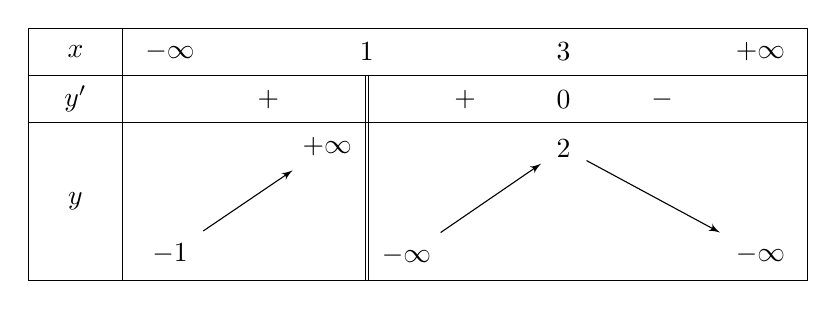
\begin{tikzpicture}
\tkzTabInit[nocadre=false,lgt=1.2,espcl=2.5,deltacl=0.6]{$x$ /0.6, $y'$ /0.6, $y$ /2}{$-\infty$, $1$, $3$, $+\infty$}
\tkzTabLine{, +, d, +, 0, -, }
\tkzTabVar{-/ $-1$, +D-/ $+\infty$ / $-\infty$, +/ $2$, -/ $-\infty$}
\end{tikzpicture}
\end{center}
Hàm số đồng biến trên khoảng nào trong các khoảng dưới đây?
\choice
{\True $(2;3)$}
{$(0;3)$}
{$(-1;2)$}
{$(3;4)$}
\loigiai{
\begin{bodembox}
\begin{itemize}
    \item Hàm số đồng biến trên khoảng $K$ nếu $y' > 0$ với mọi $x \in K$ (hoặc $y' \ge 0$ và bằng $0$ tại hữu hạn điểm trên $K$).
    \item Trên bảng biến thiên, khoảng đồng biến tương ứng với khoảng mà $y'$ mang dấu "$+$" và đồ thị (mũi tên của $y$) đi lên.
    \item Nếu một khoảng con nằm hoàn toàn trong một khoảng đồng biến thì hàm số cũng đồng biến trên khoảng con đó.
\end{itemize}
\end{bodembox}
\begin{apdungbox}
Dựa vào bảng biến thiên, ta thấy $y' > 0$ trên các khoảng $(-\infty; 1)$ và $(1; 3)$.
Do đó, hàm số đồng biến trên từng khoảng $(-\infty; 1)$ và $(1; 3)$.

Xét các đáp án:
\begin{itemize}
    \item Khoảng $(2;3)$ là tập con của khoảng $(1;3)$ nên hàm số đồng biến trên khoảng $(2;3)$.
    \item Khoảng $(0;3)$ chứa điểm $x=1$ mà tại đó hàm số không xác định nên loại.
    \item Khoảng $(-1;2)$ cũng chứa điểm $x=1$ nên loại.
    \item Trên khoảng $(3;4)$, ta thấy $y' < 0$ nên hàm số nghịch biến, loại.
\end{itemize}
Vậy đáp án đúng là $(2;3)$.
\end{apdungbox}
}
\end{ex}
\begin{ex}
Cho hình chóp $S.ABCD$ có đáy $ABCD$ là hình chữ nhật và $SA \perp (ABCD)$. Đường thẳng $SA$ không vuông góc với đường thẳng nào trong các đường thẳng sau?
\choice
{\True $SC$}
{$AB$}
{$AC$}
{$BD$}
\loigiai{
\begin{bodembox}
Định nghĩa đường thẳng vuông góc với mặt phẳng: Nếu một đường thẳng $d$ vuông góc với mặt phẳng $(\alpha)$ thì nó vuông góc với mọi đường thẳng nằm trong mặt phẳng $(\alpha)$.
Tức là: $\heva{& d \perp (\alpha) \\ & a \subset (\alpha)} \implies d \perp a$.
\end{bodembox}
\begin{apdungbox}
Theo giả thiết, ta có $SA \perp (ABCD)$.
Mà các đường thẳng $AB, AC, BD$ đều là các đường thẳng nằm trong mặt phẳng đáy $(ABCD)$.
Do đó, $SA$ vuông góc với cả ba đường thẳng $AB, AC$ và $BD$.

Xét tam giác $SAC$, vì $SA \perp AC$ nên $\Delta SAC$ vuông tại $A$. Trong một tam giác vuông chỉ có một góc vuông, do đó góc $\widehat{ASC}$ là góc nhọn, suy ra $SA$ không vuông góc với $SC$.

\begin{center}
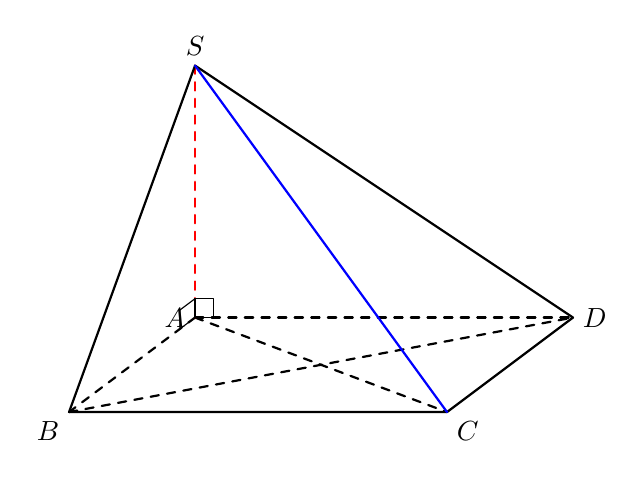
\begin{tikzpicture}[scale=0.8, >=stealth, line join=round, line cap=round]
    % Đáy ABCD
    \coordinate (A) at (0,0);
    \coordinate (B) at (-2,-1.5);
    \coordinate (C) at (4,-1.5);
    \coordinate (D) at (6,0);
    % Đỉnh S
    \coordinate (S) at (0,4);
    
    % Các đường nét đứt
    \draw[dashed, thick] (A) -- (B);
    \draw[dashed, thick] (A) -- (D);
    \draw[dashed, thick] (A) -- (C);
    \draw[dashed, thick] (B) -- (D);
    \draw[dashed, thick, red] (S) -- (A); % Chiều cao SA
    
    % Các đường nét liền
    \draw[thick] (S) -- (B) -- (C) -- (D) -- cycle;
    \draw[thick, blue] (S) -- (C); % Cạnh SC
    
    % Ký hiệu góc vuông
    \tkzMarkRightAngle[size=0.3](S,A,D);
    \tkzMarkRightAngle[size=0.3](S,A,B);
    
    % Gắn nhãn
    \node[left] at (A) {$A$};
    \node[below left] at (B) {$B$};
    \node[below right] at (C) {$C$};
    \node[right] at (D) {$D$};
    \node[above] at (S) {$S$};
\end{tikzpicture}
\end{center}
\end{apdungbox}
}
\end{ex}
\begin{ex}
Xác định tiệm cận đứng của đồ thị hàm số $y = \dfrac{ax+b}{cx+d}$ có dạng như hình dưới.
\begin{center}
\begin{tikzpicture}[>=stealth, scale=0.8, font=\footnotesize]
    % Hệ trục tọa độ
    \draw[->] (-4,0) -- (3,0) node[below] {$x$};
    \draw[->] (0,-3) -- (0,3) node[right] {$y$};
    \node[below left] at (0,0) {$O$};
    
    % Đường tiệm cận
    \draw[dashed, thick, red] (-1,-3) -- (-1,3); % Tiệm cận đứng
    \draw[dashed, thick, blue] (-4,1) -- (3,1); % Tiệm cận ngang
    
    % Vạch tọa độ
    \draw (-1,0.1) -- (-1,-0.1) node[below right] {$-1$};
    \draw (1,0.1) -- (1,-0.1) node[below] {$1$};
    \draw (0.1,1) -- (-0.1,1) node[above left] {$1$};
    \draw (0.1,-1) -- (-0.1,-1) node[right] {$-1$};
    \draw (0.1,-2) -- (-0.1,-2) node[right] {$-2$};
    
    % Vẽ đồ thị hàm phân thức
    \clip (-4,-3) rectangle (3,3);
    \draw[thick, samples=100, domain=-4:-1.1] plot (\x, {(\x - 2)/(\x + 1)});
    \draw[thick, samples=100, domain=-0.9:3] plot (\x, {(\x - 2)/(\x + 1)});
\end{tikzpicture}
\end{center}
\choice
{$x=1$}
{\True $x=-1$}
{$y=1$}
{$y=-1$}
\loigiai{
\begin{bodembox}
\begin{itemize}
    \item Đường thẳng $x = x_0$ được gọi là đường tiệm cận đứng của đồ thị hàm số $y=f(x)$ nếu ít nhất một trong các giới hạn $\lim\limits_{x \to x_0^+} f(x)$ hoặc $\lim\limits_{x \to x_0^-} f(x)$ bằng $+\infty$ hoặc $-\infty$.
    \item Nhận diện trên đồ thị: Tiệm cận đứng là đường thẳng song song với trục $Oy$ mà nhánh đồ thị tiến sát vào (vuốt dọc theo) nhưng không bao giờ cắt qua.
\end{itemize}
\end{bodembox}
\begin{apdungbox}
Quan sát đồ thị hàm số đã cho, ta thấy:
\begin{itemize}
    \item Khi $x \to (-1)^+$, nhánh đồ thị cắm thẳng xuống dưới, tức là $\lim\limits_{x \to (-1)^+} y = -\infty$.
    \item Khi $x \to (-1)^-$, nhánh đồ thị hướng thẳng lên trên, tức là $\lim\limits_{x \to (-1)^-} y = +\infty$.
\end{itemize}
Do đó, đường thẳng $x = -1$ chính là tiệm cận đứng của đồ thị hàm số.
\end{apdungbox}
}
\end{ex}
\begin{ex}
Tập nghiệm của bất phương trình $\log_2(x-2) > 2$ là
\choice
{$(4;+\infty)$}
{$(2;4)$}
{$(2;+\infty)$}
{\True $(6;+\infty)$}
\loigiai{
\begin{bodembox}
Bất phương trình logarit cơ bản:
Với cơ số $a > 1$, bất phương trình có dạng: 
\[ \log_a f(x) > b \Leftrightarrow f(x) > a^b \]
(Điều kiện $f(x) > 0$ tự động được thỏa mãn do $a^b > 0$).
\end{bodembox}
\begin{apdungbox}
Điều kiện xác định: $x - 2 > 0 \Leftrightarrow x > 2$.
Ta giải bất phương trình đã cho như sau:
\[ \log_2(x-2) > 2 \Leftrightarrow x - 2 > 2^2 \Leftrightarrow x - 2 > 4 \Leftrightarrow x > 6. \]
Kết hợp với điều kiện xác định $x > 2$, ta nhận $x > 6$.
Vậy tập nghiệm của bất phương trình là $S = (6; +\infty)$.

\begin{center}
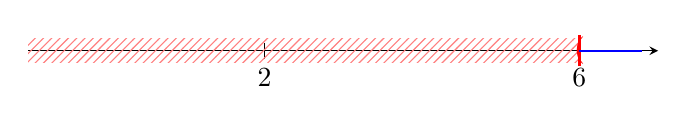
\begin{tikzpicture}[>=stealth]
    % Trục số
    \draw[->] (-1,0) -- (7,0);
    
    % Các điểm mốc
    \draw (2, 0.1) -- (2, -0.1) node[below] {$2$};
    \draw (6, 0.1) -- (6, -0.1) node[below] {$6$};
    
    % Gạch bỏ phần không thuộc tập nghiệm
    \fill[pattern=north east lines, pattern color=red!50] (-1,-0.15) rectangle (6,0.15);
    \draw[thick, red] (6,-0.2) -- (6,0.2);
    \node[red] at (6, 0) {$\mathbf{(}$};
    
    % Phần nghiệm lấy
    \draw[thick, blue] (6,0) -- (6.8,0);
\end{tikzpicture}
\end{center}
\end{apdungbox}
}
\end{ex}
\begin{ex}
Cho cấp số nhân $(u_n)$ biết $u_3 = 4$ và $u_4 = 2$. Tìm công bội $q$ của cấp số nhân đó.
\choice
{$q=2$}
{$q=4$}
{\True $q=\dfrac{1}{2}$}
{$q=\sqrt{2}$}
\loigiai{
\begin{bodembox}
Định nghĩa cấp số nhân: Cấp số nhân là một dãy số (hữu hạn hoặc vô hạn), trong đó kể từ số hạng thứ hai, mỗi số hạng đều bằng tích của số hạng đứng ngay trước nó với một hằng số $q$ không đổi. Số $q$ được gọi là công bội của cấp số nhân.
Công thức truy hồi: $u_{n+1} = u_n \cdot q \implies q = \dfrac{u_{n+1}}{u_n}$.
\end{bodembox}
\begin{apdungbox}
Áp dụng định nghĩa của cấp số nhân cho hai số hạng liên tiếp là $u_3$ và $u_4$, công bội $q$ được tính bằng:
\[ q = \dfrac{u_4}{u_3} = \dfrac{2}{4} = \dfrac{1}{2}. \]
Vậy công bội của cấp số nhân đã cho là $q = \dfrac{1}{2}$.
\end{apdungbox}
}
\end{ex}
\begin{ex}
Xác định nguyên hàm của hàm số $y=f(x)=2x^2$.
\choice
{$x^3+C$}
{\True $\dfrac{2x^3}{3}+C$}
{$\dfrac{x^3}{3}+C$}
{$6x^3+C$}
\loigiai{
\begin{bodembox}
\begin{itemize}
    \item Công thức tính nguyên hàm cơ bản của hàm số lũy thừa:
    \[ \int x^\alpha \mathrm{d}x = \dfrac{x^{\alpha+1}}{\alpha+1} + C \quad (\text{với } \alpha \ne -1). \]
    \item Tính chất đưa hằng số ra ngoài dấu nguyên hàm: 
    \[ \int k \cdot f(x) \mathrm{d}x = k \int f(x) \mathrm{d}x \quad (\text{với } k \text{ là hằng số khác } 0). \]
\end{itemize}
\end{bodembox}
\begin{apdungbox}
Áp dụng các công thức trên, ta tìm họ nguyên hàm của hàm số $f(x)$ như sau:
\[ \int f(x) \mathrm{d}x = \int 2x^2 \mathrm{d}x = 2 \int x^2 \mathrm{d}x = 2 \cdot \dfrac{x^3}{3} + C = \dfrac{2x^3}{3} + C. \]
Vậy họ nguyên hàm cần tìm là $\dfrac{2x^3}{3} + C$.
\end{apdungbox}
}
\end{ex}
\begin{ex}
Xác định tập nghiệm của phương trình $\cos x = 1$.
\choice
{\True $S = \{k2\pi \,|\, k \in \mathbb{Z}\}$}
{$S = \{\pi + k2\pi \,|\, k \in \mathbb{Z}\}$}
{$S = \{k\pi \,|\, k \in \mathbb{Z}\}$}
{$S = \{\pi + k\pi \,|\, k \in \mathbb{Z}\}$}
\loigiai{
\begin{bodembox}
Phương trình lượng giác cơ bản đối với hàm cosin ở các điểm đặc biệt biên:
\begin{itemize}
    \item $\cos x = 1 \Leftrightarrow x = k2\pi$ ($k \in \mathbb{Z}$) (Tương ứng điểm $A(1;0)$ trên đường tròn).
    \item $\cos x = -1 \Leftrightarrow x = \pi + k2\pi$ ($k \in \mathbb{Z}$).
    \item $\cos x = 0 \Leftrightarrow x = \dfrac{\pi}{2} + k\pi$ ($k \in \mathbb{Z}$).
\end{itemize}
\end{bodembox}
\begin{apdungbox}
Phương trình $\cos x = 1$ là phương trình lượng giác thuộc trường hợp đặc biệt.
Trục cosin là trục hoành. Giá trị $\cos x = 1$ đạt được tại đúng một điểm duy nhất trên đường tròn lượng giác là giao điểm của đường tròn với chiều dương trục hoành.
Điểm này ứng với góc lượng giác $x = 0 + k2\pi = k2\pi$ (với $k \in \mathbb{Z}$).

Vậy tập nghiệm của phương trình là $S = \{k2\pi \,|\, k \in \mathbb{Z}\}$.
            
\begin{center}
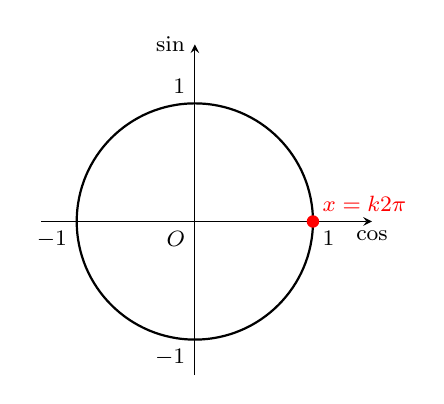
\begin{tikzpicture}[scale=1.5, >=stealth, font=\footnotesize]
    % Trục tọa độ
    \draw[->] (-1.3,0) -- (1.5,0) node[below] {$\cos$};
    \draw[->] (0,-1.3) -- (0,1.5) node[left] {$\sin$};
    \node[below left] at (0,0) {$O$};
    
    % Đường tròn lượng giác
    \draw[thick] (0,0) circle (1);
    
    % Điểm nghiệm cos x = 1
    \fill[red] (1,0) circle (1.5pt) node[above right] {$x=k2\pi$};
    \node[below right] at (1,0) {$1$};
    
    % Các điểm mốc khác
    \node[below left] at (-1,0) {$-1$};
    \node[below left] at (0,-1) {$-1$};
    \node[above left] at (0,1) {$1$};
\end{tikzpicture}
\end{center}
\end{apdungbox}
}
\end{ex}
\begin{ex}
Trong không gian với hệ tọa độ $(Oxyz)$, cho điểm $A(2;1;-2)$ và điểm $B(-4;3;4)$. Tọa độ trung điểm $M$ của đoạn $AB$ là:
\choice
{\True $(-1;2;1)$}
{$(-2;2;2)$}
{$(3;2;3)$}
{$(-2;-2;2)$}
\loigiai{
\begin{bodembox}
Cho hai điểm $A(x_A; y_A; z_A)$ và $B(x_B; y_B; z_B)$.
Tọa độ trung điểm $M$ của đoạn thẳng $AB$ được tính bởi công thức:
\[ \heva{& x_M = \dfrac{x_A + x_B}{2} \\ & y_M = \dfrac{y_A + y_B}{2} \\ & z_M = \dfrac{z_A + z_B}{2}} \]
\end{bodembox}
\begin{apdungbox}
Áp dụng công thức tính tọa độ trung điểm $M$ của đoạn thẳng $AB$:
\begin{itemize}
    \item $x_M = \displaystyle\dfrac{2 + (-4)}{2} = -1$
    \item $y_M = \displaystyle\dfrac{1 + 3}{2} = 2$
    \item $z_M = \displaystyle\dfrac{-2 + 4}{2} = 1$
\end{itemize}
Vậy tọa độ trung điểm là $M(-1; 2; 1)$.
\begin{center}
\begin{tikzpicture}[>=stealth, scale=1]
    \coordinate (A) at (0,0);
    \coordinate (B) at (4,2);
    \coordinate (M) at ($(A)!0.5!(B)$);
    
    \draw[thick] (A) -- (B);
    \fill (A) circle (2pt) node[below left] {$A(2;1;-2)$};
    \fill (B) circle (2pt) node[above right] {$B(-4;3;4)$};
    \fill[red] (M) circle (2pt) node[above left, red] {$M(-1;2;1)$};
    
    \tkzMarkSegments[mark=|,size=3pt,color=blue](A,M M,B);
\end{tikzpicture}
\end{center}
\end{apdungbox}
}
\end{ex}
\begin{ex}
Trong không gian $Oxyz$, cho mặt phẳng $(P)$ có phương trình $x-3y+5=0$. Xác định vectơ pháp tuyến của mặt phẳng $(P)$.
\choice
{\True $\vec{n}=(1;-3;0)$}
{$\vec{n}=(1;0;-3)$}
{$\vec{n}=(1;-3;5)$}
{$\vec{n}=(1;0;5)$}
\loigiai{
\begin{bodembox}
Phương trình tổng quát của mặt phẳng $(P)$ có dạng: $Ax + By + Cz + D = 0$.
Vectơ pháp tuyến của mặt phẳng $(P)$ là $\vec{n} = (A; B; C)$.
\end{bodembox}
\begin{apdungbox}
Mặt phẳng $(P) \colon x - 3y + 5 = 0$ có thể viết lại dưới dạng đầy đủ là:
\[ 1 \cdot x - 3 \cdot y + 0 \cdot z + 5 = 0 \]
Từ đó, ta xác định được các hệ số $A = 1$, $B = -3$, $C = 0$.
Suy ra vectơ pháp tuyến của mặt phẳng $(P)$ là $\vec{n} = (1; -3; 0)$.
\begin{center}
\begin{tikzpicture}[>=stealth, scale=0.8]
    \draw[thick, fill=blue!10] (0,0) -- (4,0) -- (5,2) -- (1,2) -- cycle;
    \node at (4.2, 1.8) {$(P)$};
    \coordinate (M) at (2.5,1);
    \draw[->, thick, red] (M) -- ++(0,2) node[above] {$\vec{n} = (1;-3;0)$};
    \fill (M) circle (1.5pt);
    \tkzMarkRightAngle[size=0.25](M,M,M);
    \draw (M) ++(0.25,0) -- ++(0,0.25) -- ++(-0.25,0);
\end{tikzpicture}
\end{center}
\end{apdungbox}
}
\end{ex}
\begin{ex}
Gieo một con xúc xắc cân đối và đồng chất một lần. Tính xác suất để xúc xắc xuất hiện mặt có số chấm là một số chia hết cho 3.
\choice
{\True $\dfrac{1}{3}$}
{$\dfrac{1}{2}$}
{$\dfrac{1}{6}$}
{$\dfrac{1}{4}$}
\loigiai{
\begin{bodembox}
Xác suất của biến cố $A$ được tính theo công thức cổ điển:
\[ P(A) = \dfrac{n(A)}{n(\Omega)} \]
Trong đó:
\begin{itemize}
    \item $n(\Omega)$ là số kết quả có thể xảy ra của không gian mẫu.
    \item $n(A)$ là số kết quả thuận lợi cho biến cố $A$.
\end{itemize}
\end{bodembox}
\begin{apdungbox}
Phép thử: Gieo một con xúc xắc cân đối và đồng chất 1 lần.
Không gian mẫu là tập hợp các mặt có thể xuất hiện: $\Omega = \{1; 2; 3; 4; 5; 6\}$.
Số phần tử của không gian mẫu là $n(\Omega) = 6$.

Gọi $A$ là biến cố: "Xúc xắc xuất hiện mặt có số chấm chia hết cho 3".
Các kết quả thuận lợi cho biến cố $A$ là các mặt có số chấm 3 và 6.
Tập hợp các kết quả thuận lợi: $A = \{3; 6\}$.
Số phần tử của biến cố $A$ là $n(A) = 2$.

Xác suất của biến cố $A$ là:
\[ P(A) = \displaystyle\dfrac{n(A)}{n(\Omega)} = \dfrac{2}{6} = \dfrac{1}{3} \]
\begin{center}
\begin{tikzpicture}[scale=0.6, line join=round, line cap=round]
    % Xúc xắc mặt 3
    \begin{scope}[shift={(0,0)}]
        \draw[thick, fill=white, rounded corners=2pt] (0,0) rectangle (2,2);
        \fill (0.5,0.5) circle (3pt);
        \fill (1,1) circle (3pt);
        \fill (1.5,1.5) circle (3pt);
        \node[below] at (1,-0.5) {Mặt 3 chấm};
    \end{scope}
    % Xúc xắc mặt 6
    \begin{scope}[shift={(4,0)}]
        \draw[thick, fill=white, rounded corners=2pt] (0,0) rectangle (2,2);
        \fill (0.5,0.4) circle (3pt);
        \fill (0.5,1) circle (3pt);
        \fill (0.5,1.6) circle (3pt);
        \fill (1.5,0.4) circle (3pt);
        \fill (1.5,1) circle (3pt);
        \fill (1.5,1.6) circle (3pt);
        \node[below] at (1,-0.5) {Mặt 6 chấm};
    \end{scope}
\end{tikzpicture}
\end{center}
\end{apdungbox}
}
\end{ex}
\begin{ex}
Xác định giá trị nhỏ nhất trên đoạn $[-1;1]$ của hàm số $y=f(x)$ có đồ thị như hình dưới.
\begin{center}
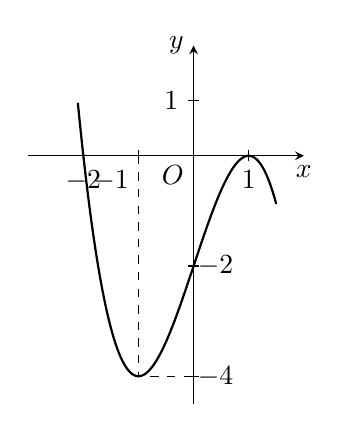
\begin{tikzpicture}[>=stealth, scale=0.7]
    % Axis
    \draw[->] (-3,0) -- (2,0) node[below] {$x$};
    \draw[->] (0,-4.5) -- (0,2) node[left] {$y$};
    \node[below left] at (0,0) {$O$};
    
    % Ticks
    \draw (-1,0.1) -- (-1,-0.1) node[below left] {$-1$};
    \draw (-2,0.1) -- (-2,-0.1) node[below] {$-2$};
    \draw (1,0.1) -- (1,-0.1) node[below] {$1$};
    \draw (0.1,1) -- (-0.1,1) node[left] {$1$};
    \draw (0.1,-2) -- (-0.1,-2) node[right] {$-2$};
    \draw (0.1,-4) -- (-0.1,-4) node[right] {$-4$};
    
    % Dashed lines
    \draw[dashed] (-1,0) -- (-1,-4) -- (0,-4);
    
    % Graph y = -x^3 + 3x - 2 (Hàm số tương ứng với đồ thị)
    \draw[thick, samples=100, domain=-2.1:1.5] plot (\x, {-\x*\x*\x + 3*\x - 2});
\end{tikzpicture}
\end{center}
\choice
{$-1$}
{\True $-4$}
{$0$}
{$-2$}
\loigiai{
\begin{bodembox}
Dựa vào đồ thị hàm số trên đoạn $[a;b]$:
\begin{itemize}
    \item Điểm thấp nhất của đồ thị trên đoạn đó tương ứng với giá trị nhỏ nhất của hàm số.
    \item Tung độ của điểm đó chính là giá trị nhỏ nhất cần tìm.
\end{itemize}
\end{bodembox}
\begin{apdungbox}
Quan sát đồ thị hàm số $y=f(x)$ trên đoạn $[-1; 1]$, ta xét tung độ các điểm thuộc đồ thị có hoành độ từ $x=-1$ đến $x=1$:
\begin{itemize}
    \item Tại $x = -1$, đồ thị đạt điểm thấp nhất (cũng là một cực tiểu của hàm số) với tung độ $y = -4$.
    \item Khi $x$ tăng từ $-1$ đến $1$, đồ thị đi lên liên tục và đạt cực đại tại điểm $(1; 0)$.
\end{itemize}
Như vậy, phần đồ thị ứng với $x \in [-1; 1]$ nằm trọn vẹn giữa tung độ thấp nhất là $-4$ và tung độ cao nhất là $0$.
Suy ra giá trị nhỏ nhất của hàm số trên đoạn $[-1; 1]$ là $y = -4$, đạt được khi $x = -1$.
\end{apdungbox}
}
\end{ex}
\begin{ex}
Mỗi ngày bác Bình đều đi bộ để rèn luyện sức khỏe. Quãng đường đi bộ mỗi ngày (đơn vị: km) của bác Bình trong 20 ngày được thống kê ở bảng sau:
\begin{center}
\begin{tabular}{|l|c|c|c|c|c|}
\hline
Quãng đường & $[2;3)$ & $[3;4)$ & $[4;5)$ & $[5;6)$ & $[6;7)$ \\
\hline
Số ngày & 3 & 6 & 5 & 4 & 2 \\
\hline
\end{tabular}
\end{center}
Khoảng biến thiên của mẫu số liệu ghép nhóm trên bằng
\choice
{7}
{6}
{1}
{\True 5}
\loigiai{
\begin{bodembox}
Đối với mẫu số liệu ghép nhóm, khoảng biến thiên, kí hiệu là $R$, là hiệu số giữa đầu mút phải của nhóm cuối cùng và đầu mút trái của nhóm đầu tiên chứa dữ liệu.
\[ R = a_{k+1} - a_1 \]
\end{bodembox}
\begin{apdungbox}
Từ bảng thống kê, ta xác định được:
\begin{itemize}
    \item Nhóm đầu tiên là $[2; 3)$, có đầu mút trái $a_1 = 2$.
    \item Nhóm cuối cùng là $[6; 7)$, có đầu mút phải $a_6 = 7$.
\end{itemize}
Khoảng biến thiên của mẫu số liệu ghép nhóm là:
\[ R = 7 - 2 = 5 \]
\end{apdungbox}
}
\end{ex}
\Closesolutionfile{ans}
\subsection*{PHẦN II. Trắc nghiệm đúng sai. (4 câu)}
\setcounter{ex}{0}
\Opensolutionfile{ans}[ans/ans-phanII]
\begin{ex}
Cho hàm số $y=f(x)=\dfrac{x^2-5x+4}{x-5}$ với $x \ne 5$.
\choiceTF
{\True $f'(x)=1-\dfrac{4}{(x-5)^2}$ với mọi $x \ne 5$.}
{\True Đồ thị hàm số cắt trục hoành tại hai điểm phân biệt.}
{\True Hàm số đạt cực đại tại $x=3$.}
{Giá trị cực tiểu bằng $3$.}
\loigiai{
\begin{bodembox}
Khảo sát hàm số phân thức:
\begin{itemize}
    \item Để tính đạo hàm nhanh hơn, ta thực hiện chia đa thức tử cho đa thức mẫu để viết về dạng $y = ax+b + \dfrac{c}{x-d}$.
    \item Giao điểm với trục hoành là nghiệm của phương trình $y=0$ (nghiệm của tử số, phải thoả mãn ĐKXĐ).
    \item Điểm cực trị thỏa mãn $y'=0$ và đổi dấu qua nghiệm. Hàm số đạt cực đại khi $y'$ đổi dấu từ $+$ sang $-$. Hàm số đạt cực tiểu khi $y'$ đổi dấu từ $-$ sang $+$.
\end{itemize}
\end{bodembox}
\begin{apdungbox}
Ta có $y = f(x) = \dfrac{x^2-5x+4}{x-5}$.
Thực hiện phép chia đa thức: $\displaystyle \dfrac{x(x-5)+4}{x-5} = x + \dfrac{4}{x-5}$.
\begin{itemize}
    \item[a)] Đạo hàm của hàm số là: 
    $\displaystyle f'(x) = 1 - \dfrac{4}{(x-5)^2}$ với mọi $x \ne 5$.
    \textbf{$\Rightarrow$ Đúng}.
    
    \item[b)] Phương trình hoành độ giao điểm với trục hoành:
    $f(x) = 0 \Leftrightarrow x^2-5x+4 = 0 \Leftrightarrow \hoac{&x=1 \\ &x=4}$.
    Vì cả hai nghiệm $x=1$ và $x=4$ đều thỏa mãn điều kiện $x \ne 5$ nên đồ thị cắt trục hoành tại 2 điểm phân biệt tọa độ là $(1;0)$ và $(4;0)$.
    \textbf{$\Rightarrow$ Đúng}.
    
    \item[c)] Xét dấu đạo hàm:
    $f'(x) = 0 \Leftrightarrow 1 - \dfrac{4}{(x-5)^2} = 0 \Leftrightarrow (x-5)^2 = 4 \Leftrightarrow \hoac{&x-5 = 2 \\ &x-5 = -2} \Leftrightarrow \hoac{&x = 7 \\ &x = 3}$.
    Bảng biến thiên:
    \begin{center}
    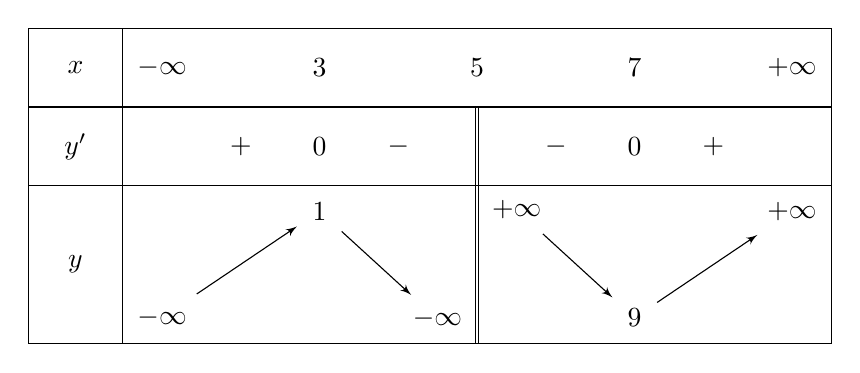
\begin{tikzpicture}
    \tkzTabInit[lgt=1.2,espcl=2]{$x$ /1, $y'$ /1, $y$ /2}{$-\infty$, $3$, $5$, $7$, $+\infty$}
    \tkzTabLine{, +, 0, -, d, -, 0, +, }
    \tkzTabVar{-/ $-\infty$, +/ $1$, -D+/ $-\infty$ / $+\infty$, -/ $9$, +/ $+\infty$}
    \end{tikzpicture}
    \end{center}
    Dựa vào bảng biến thiên, đạo hàm đổi dấu từ $+$ sang $-$ khi qua $x=3$, do đó hàm số đạt cực đại tại $x=3$.
    \textbf{$\Rightarrow$ Đúng}.
    
    \item[d)] Dựa vào bảng biến thiên, hàm số đạt cực tiểu tại $x=7$. 
    Giá trị cực tiểu tại điểm này là $f(7) = 7 + \dfrac{4}{7-5} = 9$.
    Phát biểu cho giá trị cực tiểu bằng $3$ là sai.
    \textbf{$\Rightarrow$ Sai}.
\end{itemize}
\end{apdungbox}
}
\end{ex}
\begin{ex}
Một hộp có $12$ viên bi gồm $5$ bi xanh, $6$ bi đỏ và $1$ bi vàng. Hai bạn tên là Xanh và Đỏ được trọng tài mời chơi trò chơi bốc bi ngẫu nhiên từ hộp (bi đã lấy ra không bỏ lại vào hộp). Đầu tiên trọng tài bốc một viên bi, nếu là bi xanh hoặc bi đỏ thì dừng bốc, nếu là bi vàng thì trọng tài bốc thêm một viên nữa rồi dừng bốc. Sau khi trọng tài dừng bốc, viên bi trọng tài bốc màu nào thì bạn có tên màu đó sẽ được bốc một viên và ngay sau đó trò chơi dừng lại. Người chơi bốc được viên bi có màu trùng với tên của mình sẽ là người thắng cuộc, còn nếu bốc được viên bi có màu khác với tên của mình sẽ bị thua cuộc.
\choiceTF
{\True Xác suất để trọng tài bốc được bi vàng trong lần bốc đầu tiên là $\dfrac{1}{12}$.}
{Giả sử rằng ở lần bốc đầu tiên trọng tài bốc được bi xanh. Khi đó xác suất để bạn Xanh thắng là $\dfrac{5}{11}$.}
{Giả sử rằng ở lần bốc đầu tiên trọng tài bốc được bi vàng và bốc tiếp thì được bi đỏ. Khi đó xác suất để bạn Xanh thắng là $\dfrac{1}{2}$.}
{Xác suất để bạn Đỏ thắng là $\dfrac{6}{11}$.}
\loigiai{
\begin{bodembox}
\textbf{Phân tích không gian mẫu và quy tắc trò chơi:}
\begin{itemize}
    \item Hộp ban đầu có: $5$ bi Xanh (X), $6$ bi Đỏ (Đ), $1$ bi Vàng (V). Tổng cộng $12$ bi.
    \item Trọng tài bốc bi: 
    Nếu bốc lần 1 được X hoặc Đ $\to$ Dừng lại. Người có tên tương ứng sẽ bốc.
    Nếu bốc lần 1 được V $\to$ Bốc thêm lần 2 (lúc này chỉ còn X và Đ) rồi dừng lại. Viên bi bốc lần 2 màu gì thì người có tên tương ứng sẽ bốc.
    \item Điều kiện thắng: Người được quyền bốc phải bốc ra đúng viên bi có màu trùng với tên mình từ số bi còn lại trong hộp.
\end{itemize}
\end{bodembox}
\begin{apdungbox}
\begin{itemize}
    \item[a)] Trong hộp có 12 viên bi, chỉ có 1 viên bi Vàng. 
    Xác suất để trọng tài bốc trúng bi Vàng ở lần đầu tiên là $P = \dfrac{1}{12}$.
    \textbf{$\Rightarrow$ Đúng}.

    \item[b)] Giả sử trọng tài bốc được bi xanh ở lần đầu tiên. Lúc này trọng tài dừng bốc.
    Trong hộp còn lại $11$ viên bi, trong đó có: $4$ bi Xanh, $6$ bi Đỏ, $1$ bi Vàng.
    Quyền bốc thuộc về bạn Xanh. Để bạn Xanh thắng, bạn Xanh phải bốc được bi Xanh từ hộp.
    Xác suất thắng của bạn Xanh trong trường hợp này là $\dfrac{4}{11}$ (chứ không phải $\dfrac{5}{11}$).
    \textbf{$\Rightarrow$ Sai}.

    \item[c)] Giả sử trọng tài bốc được bi Vàng lần 1 và bi Đỏ lần 2. 
    Viên bi cuối cùng trọng tài bốc là màu Đỏ, do đó \textbf{quyền bốc bi thuộc về bạn Đỏ}.
    Bạn Xanh không được bốc bi, nên xác suất để bạn Xanh thắng trong trường hợp này bằng $0$.
    \textbf{$\Rightarrow$ Sai}.

    \item[d)] Ta tính tổng xác suất để bạn Đỏ thắng chung cuộc:
    \begin{itemize}
        \item \textit{Trường hợp 1:} Trọng tài bốc được bi Đỏ ngay lần đầu.
        Xác suất xảy ra TH1: $P_1 = \dfrac{6}{12} = \dfrac{1}{2}$.
        Lúc này hộp còn 11 bi (5 Đỏ). Xác suất Đỏ bốc trúng Đỏ để thắng là $\dfrac{5}{11}$.
        Xác suất Đỏ thắng ở TH1: $\dfrac{1}{2} \cdot \dfrac{5}{11} = \dfrac{5}{22}$.
        
        \item \textit{Trường hợp 2:} Trọng tài bốc bi Vàng lần 1, bốc bi Đỏ lần 2.
        Xác suất xảy ra TH2: $P_2 = \dfrac{1}{12} \cdot \dfrac{6}{11} = \dfrac{1}{22}$.
        Lúc này hộp còn 10 bi (5 Đỏ, 5 Xanh). Xác suất Đỏ bốc trúng Đỏ để thắng là $\dfrac{5}{10} = \dfrac{1}{2}$.
        Xác suất Đỏ thắng ở TH2: $\dfrac{1}{22} \cdot \dfrac{1}{2} = \dfrac{1}{44}$.
    \end{itemize}
    Tổng xác suất để bạn Đỏ thắng chung cuộc là: $P = \dfrac{5}{22} + \dfrac{1}{44} = \dfrac{11}{44} = \dfrac{1}{4}$.
    Nhận thấy $\dfrac{1}{4} \ne \dfrac{6}{11}$ (Lưu ý: $\dfrac{6}{11}$ chính là xác suất để bạn Đỏ \textit{được trao quyền chơi}, chứ không phải xác suất thắng).
    \textbf{$\Rightarrow$ Sai}.
\end{itemize}

\begin{center}
\begin{tikzpicture}[scale=0.8]
    % Draw Box
    \draw[thick, fill=brown!20, rounded corners] (0,0) rectangle (4,3);
    \node[above, font=\bfseries] at (2,3) {Hộp 12 viên bi};
    
    % Draw Balls
    \foreach \x/\y in {0.7/0.5, 1.5/0.5, 2.3/0.5, 3.1/0.5, 1.1/1.2} {
        \shade[ball color=blue] (\x,\y) circle (0.3);
    }
    \foreach \x/\y in {2.0/1.2, 2.8/1.2, 0.7/2.0, 1.5/2.0, 2.3/2.0, 3.1/2.0} {
        \shade[ball color=red] (\x,\y) circle (0.3);
    }
    \shade[ball color=yellow] (2.0, 2.6) circle (0.3);
    
    % Labels
    \node[blue, font=\bfseries] at (-1.5, 0.8) {5 Xanh};
    \node[red, font=\bfseries] at (-1.5, 1.6) {6 Đỏ};
    \node[orange, font=\bfseries] at (-1.5, 2.6) {1 Vàng};
\end{tikzpicture}
\end{center}
\end{apdungbox}
}
\end{ex}
%----Câu Số 7------%
\begin{ex}
Người ta muốn tạo một giá đỡ bằng sắt bên cạnh một bức tường có hình dạng là đoạn cong $BDN$ như hình vẽ dưới đây. Giá đỡ được gắn với tường bằng ba thanh sắt $AB, CD, MN$ cùng vuông góc với tường ($A, C, M$ thẳng hàng và nằm trên tường). Giá đỡ được xem như là một phần của đồ thị hàm số $y = \log x$ trong mặt phẳng tọa độ $(Oxy)$ với trục tung trùng với bức tường (đơn vị trên các trục tính bằng mét). Biết $AB = 10\text{ cm}$, $AM = 1{,}4\text{ m}$ và độ dài phần đồ thị của hàm số $y=f(x)$ liên tục trên đoạn $[a;b]$ được tính theo công thức $L = \displaystyle\int\limits_a^b \sqrt{1+[f'(x)]^2} \mathrm{d}x$.

\begin{center}
\begin{tikzpicture}[>=stealth, scale=1.5, font=\footnotesize, line join=round, line cap=round]
    % Tường (Trục Oy)
    \fill[pattern=north east lines, pattern color=gray!60] (-0.4,-1.5) rectangle (0,1);
    \draw[ultra thick] (0,-1.5) -- (0,1); 
    
    % Các điểm trên tường
    \fill (0,-1.2) circle (1.5pt) node[left=2pt] {$A$};
    \fill (0,0) circle (1.5pt) node[left=2pt] {$C$};
    \fill (0,0.6) circle (1.5pt) node[left=2pt] {$M$};
    
    % Các điểm trên đồ thị
    \coordinate (B) at (0.063,-1.2); % log(x)=-1.2 => x=10^-1.2
    \coordinate (D) at (1,0);
    \coordinate (N) at (3.98, 0.6); % log(x)=0.6 => x=10^0.6
    
    \fill (B) circle (1.5pt) node[right=1pt] {$B$};
    \fill (D) circle (1.5pt) node[below right] {$D$};
    \fill (N) circle (1.5pt) node[above left] {$N$};
    
    % Các thanh sắt ngang
    \draw[thick, blue] (0,-1.2) -- (B);
    \draw[thick, blue] (0,0) -- (D) node[midway, below] {Thanh sắt};
    \draw[thick, blue] (0,0.6) -- (N);
    
    % Đồ thị đoạn cong BDN
    \draw[ultra thick, red, samples=150, domain=0.06:4] plot (\x, {ln(\x)/ln(10)});
    \node[red, right] at (1.5, 0.3) {Giá đỡ cong};
    
    % Chú thích kích thước
    \draw[decorate, decoration={brace, amplitude=4pt, mirror}, thick] (-0.5,-1.2) -- (-0.5,0.6) node[midway, left=4pt] {$1{,}4\text{ m}$};
\end{tikzpicture}
\end{center}

\choiceTF
{\True Đạo hàm của hàm số $y = \log x$ là $y' = \displaystyle\dfrac{1}{x \ln 10}$.}
{\True Trong mặt phẳng tọa độ $(Oxy)$, điểm $B$ có hoành độ bằng $0{,}1$.}
{Trong mặt phẳng tọa độ $(Oxy)$, điểm $N$ có tung độ bằng $1{,}4$.}
{\True Độ dài giá đỡ bằng $2{,}97$ mét (kết quả được làm tròn đến hàng phần trăm).}
\loigiai{
\begin{bodembox}
\textbf{Phương pháp giải toán:}
\begin{itemize}
    \item \textbf{Đạo hàm hàm số logarit:} $(\log_a x)' = \displaystyle\dfrac{1}{x \ln a}$. Lưu ý ký hiệu $\log x$ mặc định là logarit thập phân $\log_{10} x$.
    \item \textbf{Thiết lập tọa độ:} Bài toán đã quy định trục $Oy$ là bức tường, các đoạn $AB, CD, MN$ vuông góc với tường nên chúng sẽ song song với trục $Ox$. Tung độ của các điểm nằm trên đường cong đồ thị được tính qua hàm số $y = \log_{10} x$.
    \item \textbf{Ứng dụng tích phân:} Độ dài cung đường cong đồ thị $y=f(x)$ trên đoạn $[a;b]$ là $L = \displaystyle\int\limits_a^b \sqrt{1+[f'(x)]^2} \mathrm{d}x$.
\end{itemize}
\end{bodembox}

\begin{apdungbox}
Ta thiết lập hệ trục tọa độ $Oxy$ với trục $Oy$ trùng với mặt tường. Khi đó, các thanh ngang $AB, CD, MN$ song song với trục $Ox$. Vì $A, C, M \in Oy$ nên hoành độ của chúng bằng $0$.
\begin{itemize}
    \item \textbf{Xét mệnh đề a):} Hàm số mô tả giá đỡ là $y = \log x$ (cơ số $10$). Đạo hàm của nó là $y' = \displaystyle\dfrac{1}{x \ln 10}$.\\
    $\Rightarrow$ \textbf{Mệnh đề a) Đúng.}

    \item \textbf{Xét mệnh đề b):} Chiều dài thanh sắt $AB = 10\text{ cm} = 0{,}1\text{ m}$. 
    Vì $AB$ vuông góc với trục $Oy$ tại $A$ và $B$ nằm trên đồ thị, nên khoảng cách từ $B$ đến trục $Oy$ chính là hoành độ của $B$. Suy ra $x_B = 0{,}1$. \\
    $\Rightarrow$ \textbf{Mệnh đề b) Đúng.}

    \item \textbf{Xét mệnh đề c):} 
    Do $B(0{,}1; y_B)$ thuộc đồ thị $y = \log x$ nên tung độ của $B$ là:
    \[ y_B = \log(0{,}1) = \log(10^{-1}) = -1 \]
    Mặt khác, $A$ là hình chiếu của $B$ lên $Oy$ nên $A(0; -1)$.
    Theo giả thiết, độ dài $AM = 1{,}4\text{ m}$. Do $M$ nằm phía trên $A$ dọc theo trục $Oy$ nên tung độ của điểm $M$ là:
    \[ y_M = y_A + AM = -1 + 1{,}4 = 0{,}4 \]
    Vì thanh $MN \perp Oy$ tại $M$ nên điểm $N$ có cùng tung độ với $M$. Tức là $y_N = 0{,}4$ (chứ không phải $1{,}4$).\\
    $\Rightarrow$ \textbf{Mệnh đề c) Sai.}

    \item \textbf{Xét mệnh đề d):} Để tính độ dài đoạn cong giá đỡ từ $B$ đến $N$, ta cần tìm hoành độ của điểm $N$.
    Vì $N(x_N; 0{,}4)$ thuộc đồ thị $y = \log x$, ta có phương trình:
    \[ \log(x_N) = 0{,}4 \Leftrightarrow x_N = 10^{0{,}4} \approx 2{,}51188 \]
    Áp dụng công thức tính độ dài đường cong, độ dài đoạn $BN$ là:
    \[ L = \displaystyle\int\limits_{0{,}1}^{10^{0{,}4}} \sqrt{1 + [y']^2} \mathrm{d}x = \displaystyle\int\limits_{0{,}1}^{10^{0{,}4}} \sqrt{1 + \left( \displaystyle\dfrac{1}{x \ln 10} \right)^2} \mathrm{d}x \]
    Sử dụng máy tính cầm tay để tính gần đúng giá trị tích phân trên, ta thu được $L \approx 2{,}974\text{ m}$.
    Làm tròn đến hàng phần trăm (hai chữ số thập phân), ta được độ dài giá đỡ là $2{,}97$ mét.\\
    $\Rightarrow$ \textbf{Mệnh đề d) Đúng.}
\end{itemize}

\begin{center}
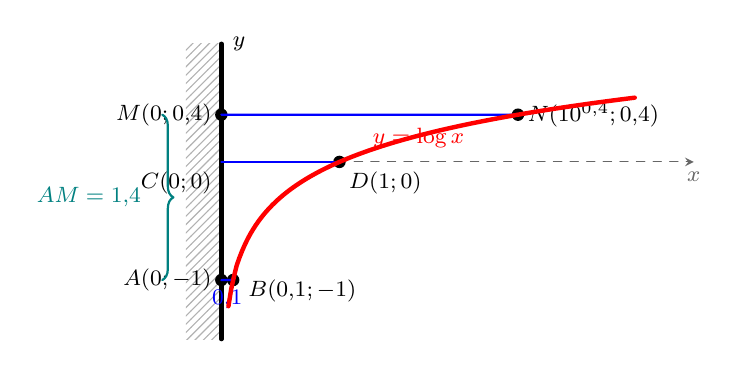
\begin{tikzpicture}[>=stealth, scale=1.5, font=\footnotesize, line join=round, line cap=round]
    % Tường (Trục Oy)
    \fill[pattern=north east lines, pattern color=gray!60] (-0.3,-1.5) rectangle (0,1);
    \draw[ultra thick] (0,-1.5) -- (0,1) node[right] {$y$};
    
    % Trục Ox
    \draw[->, dashed, gray!80!black] (0,0) -- (4,0) node[below] {$x$};
    \node[below left] at (0,0) {$C(0;0)$};
    
    % Các điểm trên Oy
    \fill (0,-1) circle (1.5pt) node[left] {$A(0;-1)$};
    \fill (0,0.4) circle (1.5pt) node[left] {$M(0;0{,}4)$};
    
    % Các điểm trên đồ thị
    \coordinate (D) at (1,0);
    \coordinate (B) at (0.1,-1);
    \coordinate (N) at (2.5118, 0.4);
    
    \fill (D) circle (1.5pt) node[below right] {$D(1;0)$};
    \fill (B) circle (1.5pt) node[right=2pt, yshift=-4pt] {$B(0{,}1;-1)$};
    \fill (N) circle (1.5pt) node[right] {$N(10^{0{,}4}; 0{,}4)$};
    
    % Các thanh sắt ngang
    \draw[thick, blue] (0,-1) -- (B) node[midway, below] {$0{,}1$};
    \draw[thick, blue] (0,0) -- (D);
    \draw[thick, blue] (0,0.4) -- (N);
    
    % Đồ thị đoạn cong
    \draw[ultra thick, red, samples=150, domain=0.06:3.5] plot (\x, {ln(\x)/ln(10)});
    \node[red, right] at (1.2, 0.2) {$y = \log x$};
    
    % Chú thích khoảng cách trên Oy
    \draw[decorate, decoration={brace, amplitude=4pt, mirror}, thick, teal] (-0.5,-1) -- (-0.5,0.4) node[midway, left=4pt] {$AM = 1{,}4$};
\end{tikzpicture}
\end{center}
\end{apdungbox}
}
\end{ex}
\begin{ex}
Trong không gian với hệ trục tọa độ $(Oxyz)$ cho điểm $A(1;2;3)$ và điểm $B(2;3;4)$. Gọi $M$ là giao điểm của đường thẳng qua hai điểm $A, B$ với mặt phẳng $(Oxy)$, $N$ thuộc trục $Oz$ sao cho $AN$ vuông góc với $AB$.
\choiceTF
{\True $\vec{AB} = (1;1;1)$.}
{Hoành độ của điểm $M$ bằng $-1$.}
{$MA = -3AB$.}
{\True $\tan \widehat{NMB} = \dfrac{\sqrt{42}}{9}$.}
\loigiai{
\begin{bodembox}
\textbf{Phương pháp giải:}
\begin{itemize}
    \item Tìm giao điểm $M$ của đường thẳng $AB$ với mặt phẳng $(Oxy) \colon z = 0$ bằng cách lập phương trình tham số.
    \item Điểm $N \in Oz \Rightarrow N(0;0;z)$. Sử dụng điều kiện vuông góc: $\vec{AN} \perp \vec{AB} \Leftrightarrow \vec{AN} \cdot \vec{AB} = 0$.
    \item Tính góc trong tam giác vuông: $\tan \alpha = \dfrac{\text{Đối}}{\text{Kề}}$.
\end{itemize}
\end{bodembox}
\begin{apdungbox}
\begin{itemize}
    \item[a)] Ta tính vectơ $\vec{AB} = (2-1; 3-2; 4-3) = (1; 1; 1)$.
    \textbf{$\Rightarrow$ Đúng}.

    \item[b)] Đường thẳng đi qua $A$ và $B$ nhận $\vec{AB}=(1;1;1)$ làm vectơ chỉ phương nên có phương trình tham số:
    $\heva{& x = 1+t \\ & y = 2+t \\ & z = 3+t}$.
    Điểm $M$ là giao điểm của $AB$ và mặt phẳng $(Oxy) \colon z = 0$ nên:
    $3+t = 0 \Leftrightarrow t = -3$.
    Thay $t = -3$ vào phương trình, ta được tọa độ $M(-2; -1; 0)$. 
    Hoành độ của $M$ là $-2$ (chứ không phải $-1$).
    \textbf{$\Rightarrow$ Sai}.

    \item[c)] Mệnh đề cho $MA = -3AB$. Khoảng cách (độ dài đoạn thẳng) thì không thể âm. 
    Nếu xét theo phương diện vectơ (thường là lỗi đánh máy thiếu dấu mũi tên), ta kiểm tra $\vec{MA}$:
    $\vec{MA} = (1 - (-2); 2 - (-1); 3 - 0) = (3; 3; 3) = 3(1; 1; 1) = 3\vec{AB}$.
    Như vậy $\vec{MA} = 3\vec{AB}$, hệ số là $3$, không phải $-3$.
    \textbf{$\Rightarrow$ Sai}.

    \item[d)] Gọi $N(0; 0; z_N) \in Oz$.
    Vectơ $\vec{AN} = (-1; -2; z_N-3)$.
    Vì $AN \perp AB$ nên $\vec{AN} \cdot \vec{AB} = 0 \Leftrightarrow (-1)(1) + (-2)(1) + (z_N-3)(1) = 0 \Leftrightarrow z_N = 6$.
    Vậy $N(0; 0; 6)$.
    Vì $M, A, B$ thẳng hàng theo thứ tự đó, nên góc $\widehat{NMB}$ chính là góc $\widehat{NMA}$.
    Tam giác $NAM$ vuông tại $A$ (do $AN \perp AB \equiv AM$).
    Độ dài các đoạn thẳng:
    $AN = |\vec{AN}| = \sqrt{(-1)^2 + (-2)^2 + (6-3)^2} = \sqrt{14}$.
    $AM = |\vec{AM}| = \sqrt{(-3)^2 + (-3)^2 + (-3)^2} = \sqrt{27} = 3\sqrt{3}$.
    $\tan \widehat{NMB} = \tan \widehat{NMA} = \dfrac{AN}{AM} = \dfrac{\sqrt{14}}{3\sqrt{3}} = \dfrac{\sqrt{42}}{9}$.
    \textbf{$\Rightarrow$ Đúng}.
\end{itemize}

\begin{center}
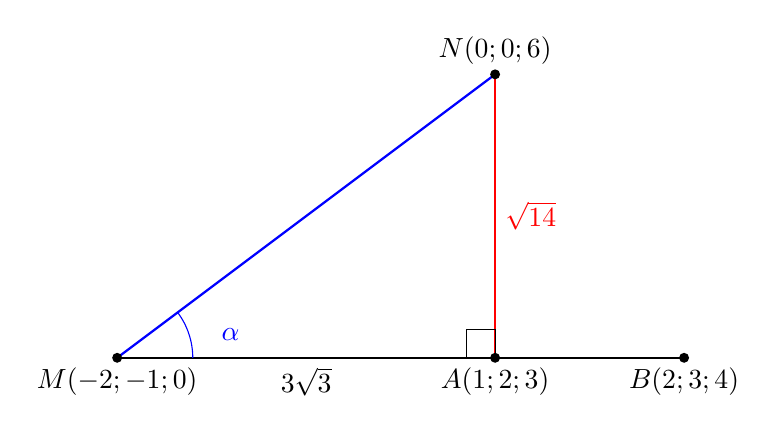
\begin{tikzpicture}[>=stealth, scale=1.2]
    \coordinate (M) at (0,0);
    \coordinate (A) at (4,0);
    \coordinate (B) at (6,0);
    \coordinate (N) at (4,3);
    
    \draw[thick] (M) -- (B);
    \draw[thick, red] (A) -- (N) node[midway, right] {$\sqrt{14}$};
    \draw[thick, blue] (M) -- (N);
    
    \fill (M) circle (1.5pt) node[below] {$M(-2;-1;0)$};
    \fill (A) circle (1.5pt) node[below] {$A(1;2;3)$};
    \fill (B) circle (1.5pt) node[below] {$B(2;3;4)$};
    \fill (N) circle (1.5pt) node[above] {$N(0;0;6)$};
    
    \tkzMarkRightAngle[size=0.3](N,A,M);
    \tkzMarkAngle[size=0.8, arc=l, color=blue](A,M,N);
    \node[blue] at (1.2, 0.25) {$\alpha$};
    \node[below] at (2,0) {$3\sqrt{3}$};
\end{tikzpicture}
\end{center}
\end{apdungbox}
}
\end{ex}
\Closesolutionfile{ans}
\subsection*{PHẦN III. Trả lời ngắn. (6 câu)}
\setcounter{ex}{0}
\Opensolutionfile{ans}[ans/ans-phanIII]
%----Câu Số 1------%
\begin{ex}
An và Bình rất giỏi Toán, cùng tham gia một trò chơi. Đầu tiên An bốc ngẫu nhiên một thẻ từ hộp thứ nhất chứa sáu thẻ giống nhau được đánh số từ $1$ đến $6$, tiếp theo Bình bốc ngẫu nhiên một thẻ từ hộp thứ hai chứa bốn thẻ giống nhau được đánh số từ $1$ đến $4$. Gọi số An bốc được là $a$ và số của Bình là $b$, sau đó hai người cùng tính giá trị của tích phân $I = \displaystyle\int\limits_{0}^{a} x^b \mathrm{d}x$. Nếu kết quả $I$ là một số nguyên thì An thắng. Ngược lại thì Bình thắng. Xác suất để An thắng là bao nhiêu? Kết quả làm tròn đến hàng phần trăm.
\shortans{0.38 }
\loigiai{
\begin{center}
\begin{tikzpicture}[>=stealth, scale=0.9, font=\small]
    % Hệ trục tọa độ mô phỏng không gian mẫu
    \draw[->, thick] (-0.5,0) -- (7.5,0) node[below] {Thẻ $a$ (An)};
    \draw[->, thick] (0,-0.5) -- (0,5.5) node[left] {Thẻ $b$ (Bình)};
    
    % Lưới điểm
    \draw[dashed, gray!40] (0,0) grid (6.5,4.5);
    \foreach \x in {1,2,3,4,5,6} \node[below] at (\x,0) {$\x$};
    \foreach \y in {1,2,3,4} \node[left] at (0,\y) {$\y$};

    % Các điểm An thắng (I nguyên) - Màu xanh
    \foreach \x/\y in {2/1, 4/1, 6/1, 3/2, 6/2, 2/3, 4/3, 6/3, 5/4} {
        \fill[green!60!black] (\x,\y) circle (0.12);
    }

    % Các điểm An thua (I không nguyên) - Dấu X đỏ
    \foreach \x/\y in {1/1, 3/1, 5/1, 1/2, 2/2, 4/2, 5/2, 1/3, 3/3, 5/3, 1/4, 2/4, 3/4, 4/4, 6/4} {
        \draw[red, thick] (\x-0.12,\y-0.12) -- (\x+0.12,\y+0.12);
        \draw[red, thick] (\x-0.12,\y+0.12) -- (\x+0.12,\y-0.12);
    }

    % Chú thích (Legend)
    \draw[thick, rounded corners, fill=yellow!10, draw=orange] (7.5, 2.5) rectangle (11.5, 4.5);
    \node[right, font=\bfseries] at (7.6, 4.1) {Không gian mẫu:};
    \fill[green!60!black] (8, 3.4) circle (0.12); 
    \node[right] at (8.3, 3.4) {An thắng ($9$ TH)};
    \draw[red, thick] (7.88, 2.68) -- (8.12, 2.92); 
    \draw[red, thick] (7.88, 2.92) -- (8.12, 2.68); 
    \node[right] at (8.3, 2.8) {An thua ($15$ TH)};
\end{tikzpicture}
\end{center}

\begin{bodembox}
\begin{itemize}
    \item \textbf{Bước 1:} Tìm số phần tử của không gian mẫu $n(\Omega)$ từ phép thử bốc thẻ của $2$ người.
    \item \textbf{Bước 2:} Tính tích phân cơ bản sử dụng công thức: $\displaystyle\int x^n \mathrm{d}x = \displaystyle\frac{x^{n+1}}{n+1} + C$.
    \item \textbf{Bước 3:} Lập luận điều kiện chia hết để $I \in \mathbb{Z}$ ứng với từng tập giá trị của $a$ và $b$, từ đó tìm số biến cố thuận lợi $n(A)$.
\end{itemize}
\end{bodembox}

\begin{apdungbox}
\begin{itemize}
    \item Không gian mẫu của phép thử là số cách bốc ngẫu nhiên $1$ thẻ từ hộp thứ nhất và $1$ thẻ từ hộp thứ hai:
    \[ n(\Omega) = 6 \times 4 = 24 \text{ (cách)} \]
    
    \item Ta tiến hành tính giá trị của tích phân $I$:
    \[ I = \displaystyle\int\limits_{0}^{a} x^b \mathrm{d}x = \left. \left( \displaystyle\frac{x^{b+1}}{b+1} \right) \right|_{0}^{a} = \displaystyle\frac{a^{b+1}}{b+1} \]
    
    \item Để An thắng thì $I$ phải là một số nguyên, điều này tương đương với việc $a^{b+1} \vdots (b+1)$.
    \item Khảo sát số bốc được của Bình là $b \in \{1; 2; 3; 4\}$, ta có các trường hợp sau:
    \begin{itemize}
        \item \textbf{Trường hợp 1:} Với $b=1 \Rightarrow b+1=2$. Ta cần $a^2 \vdots 2 \Leftrightarrow a \vdots 2$. \\
        Do $a \in \{1; 2; 3; 4; 5; 6\}$ nên $a \in \{2; 4; 6\}$ $\Rightarrow$ Có $\mathbf{3}$ cách chọn.
        
        \item \textbf{Trường hợp 2:} Với $b=2 \Rightarrow b+1=3$. Ta cần $a^3 \vdots 3 \Leftrightarrow a \vdots 3$. \\
        Suy ra $a \in \{3; 6\}$ $\Rightarrow$ Có $\mathbf{2}$ cách chọn.
        
        \item \textbf{Trường hợp 3:} Với $b=3 \Rightarrow b+1=4$. Ta cần $a^4 \vdots 4 \Leftrightarrow a^4 \vdots 2^2$. \\
        Vì phân tích thừa số nguyên tố của $a$ phải chứa số $2$, nên $a$ là số chẵn. \\
        Suy ra $a \in \{2; 4; 6\}$ $\Rightarrow$ Có $\mathbf{3}$ cách chọn (thử lại $2^4=16\,\vdots\,4$; $4^4=256\,\vdots\,4$; $6^4=1296\,\vdots\,4$ đều thỏa).
        
        \item \textbf{Trường hợp 4:} Với $b=4 \Rightarrow b+1=5$. Ta cần $a^5 \vdots 5 \Leftrightarrow a \vdots 5$. \\
        Suy ra $a \in \{5\}$ $\Rightarrow$ Có $\mathbf{1}$ cách chọn.
    \end{itemize}
    
    \item Gọi $A$ là biến cố \textit{"An thắng"}. Số các kết quả thuận lợi cho biến cố $A$ là:
    \[ n(A) = 3 + 2 + 3 + 1 = 9 \text{ (kết quả)} \]
    
    \item Vậy xác suất để An thắng trò chơi là:
    \[ P(A) = \displaystyle\frac{n(A)}{n(\Omega)} = \displaystyle\frac{9}{24} = \displaystyle\frac{3}{8} \]
\end{itemize}
\end{apdungbox}
}
\end{ex}
%----Câu Số 2------%
\begin{ex}
Dòng Hương hiền hòa trong xanh, lững lờ trôi giữa lòng thành phố Huế cổ kính và mộng mơ. Nhìn từ trên cao, hai bờ sông trải dài như hai đường thẳng song song. Cột cờ Phu Văn Lâu sừng sững cao $54{,}5$ mét như là một chứng tích hào hùng của lịch sử. Biết rằng hai bờ sông cách nhau $400$ mét và chân cột cờ (hình chiếu vuông góc của đỉnh cột cờ xuống mặt đất) nằm cách mép sông gần nhất một khoảng $200$ mét. Có hai bạn học sinh đứng ở hai bờ sông, bạn học sinh A ở cùng bờ với cột cờ nhìn đỉnh cột cờ so với mặt đất một góc $\alpha$ với $\tan\alpha = 0{,}1$ và bạn học sinh B đứng ở bờ bên kia nhìn đỉnh cột cờ so với mặt đất một góc $\beta$ với $\tan\beta = 0{,}07$. Hỏi hai bạn học sinh cách nhau xa nhất là bao nhiêu mét? (Giả sử rằng mặt đất là bằng phẳng và tầm mắt hai bạn học sinh ngang với mặt đất, kết quả làm tròn đến hàng đơn vị).
\shortans[oly]{$ 1080 $}
\loigiai{
\begin{bodembox}
\textbf{Mô hình hóa hình học bài toán:}
\begin{itemize}
    \item Gọi $S$ là đỉnh cột cờ, $H$ là chân cột cờ. Do $H$ là hình chiếu vuông góc của $S$ lên mặt đất nên $SH \perp (\text{mặt đất})$ và chiều cao cột cờ là $SH = 54{,}5 \text{ (m)}$.
    \item Vì các bạn học sinh $A, B$ đứng trên mặt đất nên các tam giác $SHA$ và $SHB$ là các tam giác vuông tại $H$.
    \item Khoảng cách từ chân cột cờ đến vị trí đứng của người quan sát được tính bằng hệ thức lượng trong tam giác vuông: $HM = \dfrac{SH}{\tan \widehat{SMH}}$.
    \item Đưa bài toán về mặt phẳng 2D (mặt đất), gắn hệ trục tọa độ $Oxy$ để tối ưu hóa khoảng cách giữa hai điểm di động trên hai đường thẳng song song.
\end{itemize}
\end{bodembox}

\begin{apdungbox}
\begin{center}
\begin{tikzpicture}[>=stealth, scale=0.85, font=\small, line join=round, line cap=round]
    % ----- BỨC TRANH 1: Góc nhìn theo mặt cắt đứng -----
    \begin{scope}[xshift=-7.5cm, yshift=1cm]
        \draw[->, gray] (-1,0) -- (5,0) node[below, black] {Mặt đất};
        \draw[->, gray] (0,-0.5) -- (0,4.5) node[left, black] {$z$ (Chiều cao)};
        
        \coordinate (H1) at (0,0);
        \coordinate (S1) at (0,3.5);
        \coordinate (A1) at (2.5,0);
        \coordinate (B1) at (4.2,0);

        % Vẽ cột cờ và tia nhìn
        \draw[ultra thick, blue] (H1) -- (S1) node[midway, left] {$54{,}5$m} node[above] {$S$};
        \fill (H1) circle (1.5pt) node[below left] {$H$};
        \draw[thick, orange] (S1) -- (A1);
        \draw[thick, teal] (S1) -- (B1);
        
        \fill (A1) circle (1.5pt) node[below] {$A$};
        \fill (B1) circle (1.5pt) node[below] {$B$};
        
        % Ký hiệu góc
        \draw (0.3,0) |- (0,0.3); % Góc vuông
        \draw (2.0,0) arc (180:125:0.5) node[left=1pt, yshift=4pt] {$\alpha$};
        \draw (3.6,0) arc (180:140:0.6) node[left=1pt, yshift=3pt] {$\beta$};
        \node at (2,-1.2) {\textit{Minh họa góc nhìn từ mặt đất}};
    \end{scope}

    % ----- BỨC TRANH 2: Hình chiếu mặt đất Oxy -----
    \begin{scope}[xshift=2cm]
        % Dòng sông
        \fill[cyan!10] (-5,2) rectangle (5,6);
        \draw[thick, blue] (-5,2) -- (5,2) node[right, black] {Bờ $d_1$ ($y=200$)};
        \draw[thick, blue] (-5,6) -- (5,6) node[right, black] {Bờ $d_2$ ($y=600$)};
        
        % Trục tọa độ
        \draw[->, dashed, gray!80!black] (-5.5,0) -- (5.5,0) node[below, black] {$x$};
        \draw[->, dashed, gray!80!black] (0,-1) -- (0,7) node[left, black] {$y$};
        \fill (0,0) circle (2pt) node[below left] {$H(0;0)$};
        
        % Điểm A và B (Tỷ lệ thu nhỏ trên hình để dễ quan sát)
        \coordinate (A) at (4.2, 2); 
        \coordinate (B) at (-4.1, 6); 
        \fill[red] (A) circle (2pt) node[above right] {$A$};
        \fill[red] (B) circle (2pt) node[below left] {$B$};
        
        % Các đoạn thẳng khoảng cách
        \draw[thick, orange] (0,0) -- (A) node[midway, below right] {$HA$};
        \draw[thick, teal] (0,0) -- (B) node[midway, left=2pt] {$HB$};
        \draw[thick, magenta] (A) -- (B) node[midway, sloped, above] {$AB_{\max}$};
        
        % Ký hiệu khoảng cách y
        \draw[<->, dashed] (-1,0) -- (-1,2) node[midway, left] {$200$};
        \draw[<->, dashed] (-1,2) -- (-1,6) node[midway, left] {$400$};
        \node at (0,-1.2) {\textit{Mặt phẳng tọa độ mặt đất ($Oxy$)}};
    \end{scope}
\end{tikzpicture}
\end{center}

\textbf{Bước 1: Tính khoảng cách từ chân cột cờ đến mỗi bạn.}
\begin{itemize}
    \item Xét tam giác vuông $SHA$, ta có khoảng cách từ $A$ đến $H$:
    \[ HA = \dfrac{SH}{\tan\alpha} = \dfrac{54{,}5}{0{,}1} = 545 \text{ (m)} \]
    \item Xét tam giác vuông $SHB$, ta có khoảng cách từ $B$ đến $H$:
    \[ HB = \dfrac{SH}{\tan\beta} = \dfrac{54{,}5}{0{,}07} = \dfrac{5450}{7} \approx 778{,}57 \text{ (m)} \]
\end{itemize}

\textbf{Bước 2: Tọa độ hóa bài toán trên mặt phẳng mặt đất.}
\begin{itemize}
    \item Gắn hệ trục tọa độ $Oxy$ trên mặt đất sao cho gốc tọa độ trùng với chân cột cờ $H(0;0)$. Trục $Oy$ vuông góc và hướng về phía bờ sông.
    \item Bờ sông thứ nhất (nơi bạn A đứng, bờ gần $H$ nhất) cách $H$ một khoảng $200\text{ m}$ nên có phương trình $d_1 \colon y = 200$.
    \item Bờ sông thứ hai (nơi bạn B đứng) cách bờ $d_1$ một khoảng $400\text{ m}$ và nằm xa $H$ hơn nên có phương trình $d_2 \colon y = 200 + 400 = 600$.
    \item Vị trí bạn A là điểm $A(x_A; 200) \in d_1$. Ta có:
    \[ HA^2 = x_A^2 + 200^2 = 545^2 \implies x_A^2 = 257025 \implies x_A \approx \pm 506{,}98 \]
    \item Vị trí bạn B là điểm $B(x_B; 600) \in d_2$. Ta có:
    \[ HB^2 = x_B^2 + 600^2 = \left(\dfrac{5450}{7}\right)^2 \implies x_B^2 = \dfrac{12062500}{49} \implies x_B \approx \pm 496{,}16 \]
\end{itemize}

\textbf{Bước 3: Tìm khoảng cách lớn nhất.}
\begin{itemize}
    \item Khoảng cách giữa hai bạn là độ dài đoạn thẳng $AB$:
    \[ AB = \sqrt{(x_A - x_B)^2 + (y_A - y_B)^2} = \sqrt{(x_A - x_B)^2 + 400^2} \]
    \item Để $AB$ đạt giá trị lớn nhất, biểu thức $\Delta x^2 = (x_A - x_B)^2$ phải lớn nhất. Điều này chỉ xảy ra khi $x_A$ và $x_B$ mang dấu trái ngược nhau (tức là hai bạn đứng ở hai phía đối diện nhau so với trục $Oy$).
    \item Giả sử chọn $x_A > 0$ và $x_B < 0$, ta có $\Delta x_{\max} = |x_A| + |x_B| \approx 506{,}98 + 496{,}16 = 1003{,}14$.
    \item Thay vào công thức, khoảng cách lớn nhất là:
    \[ AB_{\max} = \sqrt{(1003{,}14)^2 + 400^2} \approx \sqrt{1006290 + 160000} = \sqrt{1166290} \approx 1079{,}95 \text{ (m)} \]
    \item Theo yêu cầu làm tròn đến hàng đơn vị, kết quả thu được là \textbf{1080} (mét).
\end{itemize}
\end{apdungbox}
}
\end{ex}
%----Câu Số 3------%
\begin{ex}
Đất sét là một dạng vật chất đặc và mềm, có thể tạo thành nhiều hình dạng khác nhau nhưng thể tích không đổi. Đầu tiên ta có một cục đất sét với thể tích $1000\text{ cm}^3$, người ta nặn thành một khối lập phương đặc, sau đó khoét phần đất sét ở giữa để tạo thành một chậu không nắp (phần trong của chậu có dạng hình hộp chữ nhật) có độ dày bốn mặt bên và độ dày đáy bằng nhau và bằng $\dfrac{1}{10}$ độ dài cạnh của khối lập phương. Phần đất sét còn dư cũng được nặn thành một khối lập phương đặc và cũng khoét phần đất sét ở giữa để tạo thành một chậu không nắp với tỉ lệ giữa độ dày của các mặt và cạnh khối lập phương như trên. Cứ tiếp tục như vậy cho đến khi được $5$ cái chậu. Tính tổng thể tích nước mà $5$ chậu đó có thể chứa (đơn vị là $\text{cm}^3$, kết quả làm tròn đến hàng đơn vị).
\shortans[oly]{$ 1272 $}
\loigiai{
\begin{bodembox}
\textbf{Phân tích cấu trúc một chậu đất sét:}
\begin{itemize}
    \item Gọi $a$ là cạnh của khối lập phương đặc. Thể tích khối lập phương ban đầu là $V = a^3$.
    \item Bề dày của mặt đáy và $4$ mặt bên đều là $t = \dfrac{a}{10} = 0{,}1a$.
    \item Do chậu không có nắp nên phần rỗng bên trong là một hình hộp chữ nhật có các kích thước:
    \[ \text{Chiều dài} = a - 2t = 0{,}8a; \quad \text{Chiều rộng} = a - 2t = 0{,}8a; \quad \text{Chiều sâu (cao)} = a - t = 0{,}9a \]
    \item Thể tích phần rỗng (chính là sức chứa nước của chậu) được tính theo thể tích ban đầu $V$:
    \[ W = 0{,}8a \times 0{,}8a \times 0{,}9a = 0{,}576a^3 = 0{,}576V \]
\end{itemize}
\end{bodembox}

\begin{apdungbox}
\begin{center}
\begin{tikzpicture}[>=stealth, scale=0.85, font=\small, line join=round, line cap=round]
    % ----- Hình 1: Lát cắt 2D minh họa mặt đứng -----
    \begin{scope}[xshift=-6cm, yshift=0.5cm]
        % Vỏ ngoài
        \draw[thick, fill=orange!50!brown] (0,0) rectangle (4,4);
        % Phần rỗng bên trong (biểu diễn nước màu xanh)
        \draw[thick, fill=cyan!15] (0.4,0.4) rectangle (3.6,4);
        
        % Ghi chú kích thước vỏ ngoài
        \draw[<->] (0,-0.6) -- (4,-0.6) node[midway, below] {$a$};
        \draw[<->] (-0.6,0) -- (-0.6,4) node[midway, left] {$a$};
        
        % Ghi chú bề dày các cạnh
        \draw[<->] (0, 0.2) -- (0.4, 0.2) node[midway, above] {$0{,}1a$};
        \draw[<->] (3.6, 0.2) -- (4, 0.2) node[midway, above] {$0{,}1a$};
        \draw[<->] (2, 0) -- (2, 0.4) node[midway, right] {$0{,}1a$};
        
        % Ghi chú lòng rỗng
        \draw[<->, dashed] (0.4, 2) -- (3.6, 2) node[midway, above] {$0{,}8a$};
        \draw[<->, dashed] (2, 0.4) -- (2, 4) node[midway, right] {$0{,}9a$};
        
        \node[below] at (2,-1.2) {\textit{Mặt cắt đứng của chậu đất sét}};
    \end{scope}

    % ----- Hình 2: 3D của khối hộp bị khoét -----
    \begin{scope}[xshift=1.5cm]
        \coordinate (O) at (0,0);
        \coordinate (A) at (4,0);
        \coordinate (B) at (5,1.5);
        \coordinate (C) at (1,1.5);
        \coordinate (T1) at (0,4);
        \coordinate (T2) at (4,4);
        \coordinate (T3) at (5,5.5);
        \coordinate (T4) at (1,5.5);
        
        % Các đỉnh rỗng phía dưới
        \coordinate (I1) at (0.4, 0.4); 
        \coordinate (I2) at (3.6, 0.4);
        \coordinate (I3) at (4.6, 1.9);
        \coordinate (I4) at (1.4, 1.9);
        
        % Các đỉnh rỗng miệng chậu
        \coordinate (TI1) at (0.4, 4);
        \coordinate (TI2) at (3.6, 4);
        \coordinate (TI3) at (4.6, 5.5);
        \coordinate (TI4) at (1.4, 5.5);
        
        % Vẽ các mặt ngoài khối chậu
        \draw[thick, fill=orange!50!brown] (O)--(A)--(T2)--(T1)--cycle; % Mặt trước
        \draw[thick, fill=orange!70!brown] (A)--(B)--(T3)--(T2)--cycle; % Mặt bên phải
        \draw[thick, fill=orange!30!brown] (T1)--(T2)--(T3)--(T4)--cycle; % Mặt trên (bề dày)
        
        % Vẽ phần khoét lỗ (đổ màu không gian bên trong)
        \draw[thick, fill=cyan!15] (TI1)--(TI2)--(TI3)--(TI4)--cycle; % Mặt thoáng
        \draw[thick, fill=cyan!10] (TI1)--(TI2)--(I2)--(I1)--cycle; % Thành trong mặt trước
        \draw[thick, fill=cyan!30] (TI2)--(TI3)--(I3)--(I2)--cycle; % Thành trong mặt phải
        
        % Các nét khuất phía sau
        \draw[dashed, thick, gray!80] (O)--(C)--(B) (C)--(T4);
        \draw[dashed, thick, gray!80] (TI4)--(I4) (I1)--(I4)--(I3);
        
        % Nhãn kích thước khối ngoài
        \node[below] at (2,0) {$a$};
        \node[left] at (0,2) {$a$};
        \node[align=center] at (2.5, 6.2) {\textit{Mô hình 3D khối lập phương bị khoét}};
    \end{scope}
\end{tikzpicture}
\end{center}

\begin{itemize}
    \item Khi khoét phần giữa để tạo chậu, phần đất sét dư được lấy ra chính là lượng đất sét chiếm chỗ nằm ở phần rỗng. Do đó, thể tích đất sét dư này để làm chậu tiếp theo sẽ có giá trị đúng bằng sức chứa nước $W$ của chiếc chậu vừa tạo.
    \item \textbf{Xét chậu thứ 1:} 
    Thể tích đất ban đầu là $V_0 = 1000$. Sức chứa của chậu $1$ là:
    \[ W_1 = 0{,}576 V_0 = 0{,}576 \times 1000 = 576 \]
    Phần đất dư để làm chậu $2$ là $V_1 = W_1 = 576$.
    
    \item \textbf{Xét chậu thứ 2:} 
    Sức chứa của chậu $2$ tính theo thể tích phần đất làm ra nó:
    \[ W_2 = 0{,}576 V_1 = 0{,}576 W_1 = 0{,}576 \times 576 = 331{,}776 \]
    
    \item Dễ thấy, dãy sức chứa của các chiếc chậu $(W_n)$ lập thành một cấp số nhân lùi với số hạng đầu $W_1 = 576$ và công bội $q = 0{,}576$.
    \item Tổng thể tích nước mà $5$ chậu có thể chứa là tổng $5$ số hạng đầu của cấp số nhân này:
    \[ S_5 = W_1 \cdot \dfrac{1 - q^5}{1 - q} = 576 \cdot \dfrac{1 - (0{,}576)^5}{1 - 0{,}576} \approx 576 \cdot \dfrac{1 - 0{,}063668}{0{,}424} \approx 1272{,}357 \text{ (cm}^3) \]
    \item Theo yêu cầu làm tròn đến hàng đơn vị, kết quả thu được là \textbf{1272}.
\end{itemize}
\end{apdungbox}
}
\end{ex}

%----Câu Số 4------%
\begin{ex}
Hằng năm trước ngày Khai giảng năm học mới, Ủy ban nhân dân thành phố Huế giao Sở Giáo dục và Đào tạo tổ chức Lễ Tuyên dương học sinh đạt danh hiệu “Học sinh danh dự toàn trường” dành cho những học sinh xuất sắc nhất của mỗi trường phổ thông trên địa bàn thành phố. Trong Lễ Tuyên dương, Ban tổ chức vinh danh các học sinh theo lượt nhận, mỗi lượt có $10$ học sinh, với những lượt có $5$ học sinh nam và $5$ học sinh nữ thì Ban tổ chức muốn các học sinh này đứng thành một hàng mà nam nữ xen kẽ. Tuy nhiên khi xếp hàng với lượt có $5$ học sinh nam và $5$ học sinh nữ thì Ban tổ chức nhận thấy các học sinh này không đứng xen kẽ nhưng chỉ cần đổi chỗ hai học sinh nào đó thì được hàng có nam nữ đứng xen kẽ, cách xếp này gọi là “cách xếp lỗi”. Gọi $D$ là số “cách xếp lỗi” như trên, xác định giá trị của $\dfrac{D}{100}$.
\shortans[oly]{$ 7200 $}
\loigiai{
\begin{bodembox}
\textbf{Sơ đồ tư duy giải toán:}
\begin{itemize}
    \item Tính tổng số cách xếp hàng đúng chuẩn nam nữ xen kẽ cho $10$ học sinh.
    \item Phân tích đặc điểm của "cách xếp lỗi": Đây là cấu hình sai khác so với một cấu hình chuẩn xen kẽ bởi đúng $1$ cặp học sinh ($1$ Nam và $1$ Nữ) bị hoán đổi vị trí.
    \item Tính số cách tạo ra "cách xếp lỗi" từ một cấu hình chuẩn và nhân với tổng số cấu hình chuẩn để thu được kết quả, do tính tương ứng $1-1$ giữa việc sửa lỗi và tạo lỗi.
\end{itemize}
\end{bodembox}

\begin{apdungbox}
\begin{center}
\begin{tikzpicture}[scale=0.85, >=stealth, font=\small, line join=round, line cap=round]
    % Xếp chuẩn
    \node[left, font=\bfseries] at (0, 2) {Hàng chuẩn:};
    \foreach \i in {1,2,3,4,5} {
        \fill[blue!15, draw=blue!60, thick] (2*\i-1, 2) circle (0.45);
        \node[blue!80!black, font=\bfseries] at (2*\i-1, 2) {Nam};
        
        \fill[pink!30, draw=pink!80, thick] (2*\i, 2) circle (0.45);
        \node[red!70!black, font=\bfseries] at (2*\i, 2) {Nữ};
    }
    
    % Hoán đổi
    \draw[<->, thick, red, dashed] (4, 1.4) .. controls (4, 0.5) and (7, 0.5) .. (7, 1.4);
    \node[red, font=\footnotesize] at (5.5, 0.3) {Hoán đổi vị trí $1$ Nam và $1$ Nữ ($C_5^1 \times C_5^1 = 25$ cách)};
    
    % Xếp lỗi
    \node[left, font=\bfseries] at (0, -1) {Hàng lỗi:};
    \foreach \i in {1,2,3,4,5} {
        \ifnum\i=2
            % Vị trí 4 ban đầu là Nữ, bị đổi thành Nam
            \fill[blue!15, draw=blue!60, thick] (2*\i, -1) circle (0.45);
            \node[blue!80!black, font=\bfseries] at (2*\i, -1) {Nam};
        \else
            \fill[pink!30, draw=pink!80, thick] (2*\i, -1) circle (0.45);
            \node[red!70!black, font=\bfseries] at (2*\i, -1) {Nữ};
        \fi
        
        \ifnum\i=4
            % Vị trí 7 ban đầu là Nam, bị đổi thành Nữ
            \fill[pink!30, draw=pink!80, thick] (2*\i-1, -1) circle (0.45);
            \node[red!70!black, font=\bfseries] at (2*\i-1, -1) {Nữ};
        \else
            \fill[blue!15, draw=blue!60, thick] (2*\i-1, -1) circle (0.45);
            \node[blue!80!black, font=\bfseries] at (2*\i-1, -1) {Nam};
        \fi
    }
    
    % Braces for error highlights
    \draw[decorate, decoration={brace, amplitude=5pt, mirror}, thick, red] (2.5, -1.6) -- (5.5, -1.6) node[midway, below=5pt] {Cụm Nam kề nhau};
    \draw[decorate, decoration={brace, amplitude=5pt, mirror}, thick, red] (5.5, -1.6) -- (8.5, -1.6) node[midway, below=5pt] {Cụm Nữ kề nhau};
\end{tikzpicture}
\end{center}

\textbf{Bước 1: Tính số cách xếp hàng đúng chuẩn xen kẽ.}
\begin{itemize}
    \item Có $2$ mô hình đứng xen kẽ đúng chuẩn:
    \begin{itemize}
        \item \textit{Mô hình 1:} (Nam - Nữ - Nam - Nữ - Nam - Nữ - Nam - Nữ - Nam - Nữ).
        \item \textit{Mô hình 2:} (Nữ - Nam - Nữ - Nam - Nữ - Nam - Nữ - Nam - Nữ - Nam).
    \end{itemize}
    \item Với mỗi mô hình, ta có $5!$ cách xếp $5$ bạn Nam vào $5$ vị trí dành cho Nam, và $5!$ cách xếp $5$ bạn Nữ vào $5$ vị trí dành cho Nữ.
    \item Tổng số cách xếp chuẩn xen kẽ là:
    \[ S = 2 \times 5! \times 5! = 2 \times 120 \times 120 = 28800 \text{ (cách)} \]
\end{itemize}

\textbf{Bước 2: Xác định số cách sinh ra "cách xếp lỗi".}
\begin{itemize}
    \item Từ một cấu hình xếp chuẩn xen kẽ bất kỳ, nếu ta chọn ra $1$ học sinh Nam và $1$ học sinh Nữ rồi hoán đổi vị trí của họ, bạn Nam sẽ rơi vào vị trí chẵn (vốn dành cho Nữ) và bạn Nữ sẽ rơi vào vị trí lẻ (vốn dành cho Nam). Việc này chắc chắn tạo ra một cấu hình phá vỡ tính xen kẽ.
    \item Số cách chọn để hoán đổi từ $1$ cấu hình chuẩn là:
    \[ C_5^1 \times C_5^1 = 5 \times 5 = 25 \text{ (cách)} \]
    \item Vì một "cách xếp lỗi" chỉ có duy nhất $1$ bạn Nam và $1$ bạn Nữ đứng sai vị trí (không xen kẽ), ta bắt buộc phải hoán đổi lại đúng $2$ bạn này để khôi phục về trạng thái chuẩn. Điều này chứng tỏ mỗi "cách xếp lỗi" chỉ được sinh ra từ đúng \textbf{một} cấu hình chuẩn duy nhất, không có sự trùng lặp.
\end{itemize}

\textbf{Bước 3: Tính toán kết quả.}
\begin{itemize}
    \item Tổng số "cách xếp lỗi" là: 
    \[ D = S \times 25 = 28800 \times 25 = 720000 \]
    \item Giá trị cần tìm theo yêu cầu bài toán là: 
    \[ \dfrac{D}{100} = \dfrac{720000}{100} = 7200 \]
\end{itemize}
\end{apdungbox}
}
\end{ex}

%----Câu Số 5------%
\begin{ex}
Một hộ sản xuất và kinh doanh một mặt hàng $A$, biết rằng chi phí để sản xuất $x\text{ kg } (x>0)$ mặt hàng $A$ là $\dfrac{2x^2+x}{x+1}$ (đơn vị triệu đồng), trong lúc đó bán ra mỗi kg là $3$ triệu đồng. Hỏi cần sản xuất bao nhiêu kg mặt hàng $A$ để lợi nhuận đạt $15$ triệu đồng (kết quả làm tròn đến hàng phần chục)?
\shortans[oly]{$ 14{,}1 $}
\loigiai{
\begin{bodembox}
\textbf{Mô hình bài toán kinh tế học:}
\begin{itemize}
    \item \textbf{Hàm doanh thu:} $R(x) = p \cdot x$ (với $p$ là đơn giá bán, $x$ là số lượng bán ra).
    \item \textbf{Hàm lợi nhuận:} $P(x) = R(x) - C(x)$ (với $C(x)$ là hàm chi phí sản xuất).
    \item Bài toán yêu cầu tìm sản lượng $x$ sao cho $P(x) = P_0$, dẫn đến việc thiết lập và giải phương trình đại số.
\end{itemize}
\end{bodembox}

\begin{apdungbox}
\textbf{Bước 1: Thiết lập hàm lợi nhuận.}
\begin{itemize}
    \item Gọi $x$ ($x > 0$) là sản lượng mặt hàng $A$ cần sản xuất (đơn vị: kg).
    \item Doanh thu khi bán ra $x$ kg với giá $3$ triệu đồng/kg là:
    \[ R(x) = 3x \text{ (triệu đồng)} \]
    \item Hàm chi phí sản xuất đã cho là:
    \[ C(x) = \dfrac{2x^2+x}{x+1} \text{ (triệu đồng)} \]
    \item Hàm lợi nhuận thu được là:
    \[ P(x) = R(x) - C(x) = 3x - \dfrac{2x^2+x}{x+1} \]
    \[ P(x) = \dfrac{3x(x+1) - (2x^2+x)}{x+1} = \dfrac{3x^2+3x - 2x^2-x}{x+1} = \dfrac{x^2+2x}{x+1} \]
\end{itemize}

\textbf{Bước 2: Giải phương trình tìm sản lượng.}
\begin{itemize}
    \item Theo giả thiết, lợi nhuận đạt $15$ triệu đồng, tức là $P(x) = 15$. Ta có phương trình:
    \[ \dfrac{x^2+2x}{x+1} = 15 \]
    \item Do $x > 0$ nên $x+1 \neq 0$, quy đồng và khử mẫu ta được:
    \[ x^2 + 2x = 15(x+1) \]
    \[ \Leftrightarrow x^2 + 2x = 15x + 15 \]
    \[ \Leftrightarrow x^2 - 13x - 15 = 0 \]
    \item Xét biệt thức $\Delta = (-13)^2 - 4 \cdot 1 \cdot (-15) = 169 + 60 = 229 > 0$. Phương trình bậc hai có hai nghiệm phân biệt:
    \[ \hoac{& x_1 = \dfrac{13 + \sqrt{229}}{2} \approx 14{,}0666... \text{ (thỏa mãn điều kiện } x > 0) \\ & x_2 = \dfrac{13 - \sqrt{229}}{2} \approx -1{,}0666... \text{ (loại vì } x > 0)} \]
    \item Làm tròn nghiệm nhận được đến hàng phần chục (chữ số thập phân thứ nhất), ta được $x \approx 14{,}1$.
    \item Vậy hộ gia đình cần sản xuất khoảng $\mathbf{14{,}1}$ kg mặt hàng A.
\end{itemize}

\begin{center}
\begin{tikzpicture}[>=stealth, x=0.65cm, y=0.35cm, font=\small, line join=round, line cap=round]
    % Trục tọa độ
    \draw[->, thick, gray!80!black] (-1,0) -- (18,0) node[below, black] {$x$ (sản lượng)};
    \draw[->, thick, gray!80!black] (0,-2) -- (0,21) node[left, black] {$P(x)$ (lợi nhuận)};
    \fill (0,0) circle (1.5pt) node[below left] {$O$};
    
    % Lưới điểm tọa độ giao
    \draw[dashed, thick, gray] (14.066, 15) -- (14.066, 0) node[below, black, font=\bfseries] {$14{,}1$};
    \draw[dashed, thick, gray] (14.066, 15) -- (0, 15) node[left, black, font=\bfseries] {$15$};
    
    % Đường cong đồ thị P(x) = (x^2+2x)/(x+1)
    \draw[ultra thick, blue, smooth, samples=150, domain=0:16.5] plot (\x, {(\x*\x + 2*\x)/(\x + 1)});
    \node[blue, right] at (14.5, 18.5) {$P(x) = \dfrac{x^2+2x}{x+1}$};
    
    % Đường thẳng mục tiêu y = 15
    \draw[thick, red] (0, 15) -- (17.5, 15) node[above left] {$y = 15$};
    
    % Điểm cắt
    \fill[red] (14.066, 15) circle (2pt) node[above left] {$M$};
    \node[below right] at (8, -2) {\textit{Đồ thị minh họa giao điểm của hàm lợi nhuận}};
\end{tikzpicture}
\end{center}
\end{apdungbox}
}
\end{ex}

%----Câu Số 6------%
\begin{ex}
Cho hình chóp cụt tam giác đều $ABC.MNP$ có đáy lớn là tam giác $ABC$ với độ dài cạnh bằng $6$, chiều cao của hình chóp cụt bằng $8$. Gọi $G$ là trọng tâm tam giác $MNP$. Tính khoảng cách giữa hai đường thẳng $AG$ và $BC$ (kết quả làm tròn đến hàng phần trăm).
\shortans[oly]{$ 4{,}77 $}
\loigiai{
\begin{bodembox}
\textbf{Phương pháp tìm khoảng cách giữa hai đường thẳng chéo nhau:}
\begin{itemize}
    \item \textbf{Phương pháp hình học thuần túy:} Dựng mặt phẳng $(\alpha)$ chứa đường thẳng này và vuông góc với đường thẳng kia. Khoảng cách cần tìm chính là khoảng cách từ giao điểm của đường thẳng vuông góc đến đường thẳng nằm trong mặt phẳng $(\alpha)$.
    \item \textbf{Hệ tọa độ phẳng hóa (2D):} Tận dụng tính đối xứng của hình chóp đều, ta thiết lập hệ trục tọa độ $Oxy$ ngay trên mặt cắt đối xứng chứa $2$ đường thẳng cần tính khoảng cách để chuyển bài toán không gian phức tạp về bài toán hình học phẳng đơn giản.
\end{itemize}
\end{bodembox}

\begin{apdungbox}
\begin{center}
\begin{tikzpicture}[>=stealth, line join=round, line cap=round, font=\small]
    % --- Mô hình 3D Hình chóp cụt ---
    \begin{scope}[xshift=-6cm, scale=0.9]
        % Tọa độ các điểm 3D (giả lập)
        \coordinate (A) at (-1.5, 2);
        \coordinate (B) at (-3, -1);
        \coordinate (C) at (3, -1);
        \coordinate (M1) at (0, -1);
        \coordinate (Gp) at (-0.5, 0);
        \coordinate (G) at (-0.5, 4);
        \coordinate (M) at (-1, 5);
        \coordinate (N) at (-1.75, 3.5);
        \coordinate (P) at (1.25, 3.5);

        % Đổ màu mặt phẳng đối xứng (AGM1)
        \fill[green!10, opacity=0.8] (A) -- (M1) -- (G) -- cycle;

        % Các nét khuất (sau)
        \draw[dashed, thick] (A) -- (B);
        \draw[dashed, thick] (A) -- (C);
        \draw[dashed, thick] (M) -- (A);
        \draw[dashed, thick] (A) -- (M1);
        \draw[dashed, thick, orange] (G) -- (Gp) node[midway, left, black] {$8$};
        \draw[dashed, thick] (Gp) -- (M1);
        \draw[dashed, ultra thick, blue] (A) -- (G);

        % Các nét thấy (trước)
        \draw[thick] (B) -- (C);
        \draw[thick] (N) -- (B);
        \draw[thick] (P) -- (C);
        \draw[thick] (M) -- (N) -- (P) -- cycle;
        \draw[thick] (G) -- (M1);

        % Vẽ các điểm
        \fill (A) circle (1.5pt) node[above left] {$A$};
        \fill (B) circle (1.5pt) node[below left] {$B$};
        \fill (C) circle (1.5pt) node[below right] {$C$};
        \fill (M1) circle (1.5pt) node[below] {$M_1$};
        \fill (Gp) circle (1.5pt) node[below right] {$G'$};
        \fill (G) circle (1.5pt) node[above right] {$G$};
        
        \node[below] at (0,-1.8) {\textit{Mô hình 3D hình chóp cụt}};
    \end{scope}

    % --- Mô hình 2D Tọa độ hóa ---
    \begin{scope}[xshift=2cm, scale=0.7]
        \coordinate (Gp) at (0,0);
        \coordinate (M1) at (1.732, 0); % sqrt(3)
        \coordinate (A) at (-3.464, 0); % -2sqrt(3)
        \coordinate (G) at (0, 5); % Scale y=8 -> 5 để hình cân đối

        % Trục tọa độ
        \draw[->, dashed, gray!80!black] (-4.5,0) -- (3,0) node[below, black] {$x$};
        \draw[->, dashed, gray!80!black] (0,-1) -- (0,6) node[left, black] {$y$};
        \fill (Gp) circle (2pt) node[below right] {$G'(0;0)$};

        % Vẽ các điểm trên mặt phẳng
        \fill (A) circle (2pt) node[below] {$A(-2\sqrt{3};0)$};
        \fill (M1) circle (2pt) node[below] {$M_1(\sqrt{3};0)$};
        \fill (G) circle (2pt) node[right] {$G(0;8)$};

        % Các đoạn thẳng
        \draw[ultra thick, blue] (A) -- (G) node[midway, sloped, above] {$AG$};
        \draw[thick] (A) -- (M1);
        \draw[thick, orange] (Gp) -- (G) node[midway, left, black] {$8$};

        % Đường vuông góc thể hiện khoảng cách
        \coordinate (H) at ($ (A)!(M1)!(G) $);
        \draw[thick, red] (M1) -- (H) node[midway, right=2pt, yshift=-4pt] {$d \approx 4{,}77$};
        
        % Ký hiệu góc vuông
        \coordinate (Hdir) at ($ (H)!0.2!(M1) $);
        \coordinate (Adir) at ($ (H)!0.2!(A) $);
        \coordinate (corner) at ($ (Hdir) + (Adir) - (H) $);
        \draw[red, thick] (Hdir) -- (corner) -- (Adir);
        \fill[red] (H) circle (1.5pt) node[above left] {$H$};

        % Braces ghi chú độ dài
        \draw[decorate, decoration={brace, amplitude=5pt, mirror}, thick] (-3.464, -0.4) -- (0, -0.4) node[midway, below=5pt] {$2\sqrt{3}$};
        \draw[decorate, decoration={brace, amplitude=5pt, mirror}, thick] (0, -0.4) -- (1.732, -0.4) node[midway, below=5pt] {$\sqrt{3}$};

        \node[below] at (-0.5,-1.8) {\textit{Mặt phẳng tọa độ cắt ngang $(AGM_1)$}};
    \end{scope}
\end{tikzpicture}
\end{center}

\textbf{Bước 1: Phân tích tính chất vuông góc và xác định mặt phẳng cắt.}
\begin{itemize}
    \item Gọi $G'$ là trọng tâm của tam giác đều đáy $ABC$. Vì $ABC.MNP$ là hình chóp cụt đều, đoạn nối hai trọng tâm $GG'$ chính là đường cao của hình chóp cụt. 
    \item Do đó $GG' \perp (ABC)$ và theo giả thiết ta có $GG' = 8$.
    \item Gọi $M_1$ là trung điểm của $BC$. Trong tam giác đều $ABC$ có cạnh $a=6$, đường trung tuyến $AM_1$ đồng thời là đường cao nên $AM_1 \perp BC$ và có độ dài:
    \[ AM_1 = \dfrac{a\sqrt{3}}{2} = \dfrac{6\sqrt{3}}{2} = 3\sqrt{3} \]
    \item Trọng tâm $G'$ nằm trên $AM_1$ sao cho ba điểm $A, G', M_1$ thẳng hàng. Theo tính chất trọng tâm:
    \[ G'A = \dfrac{2}{3} AM_1 = 2\sqrt{3} \quad \text{và} \quad G'M_1 = \dfrac{1}{3} AM_1 = \sqrt{3} \]
    \item Ta có hệ điều kiện: $\heva{& BC \perp AM_1 \\ & BC \perp GG' \text{ (do } GG' \perp (ABC))} \implies BC \perp (AGM_1)$.
    \item Do đường thẳng $AG$ nằm hoàn toàn trong mặt phẳng $(AGM_1)$, suy ra khoảng cách giữa hai đường thẳng chéo nhau $AG$ và $BC$ chính bằng khoảng cách từ điểm $M_1$ (là giao điểm của $BC$ và $(AGM_1)$) đến đường thẳng $AG$.
\end{itemize}

\textbf{Bước 2: Tọa độ hóa trong mặt phẳng $(AGM_1)$.}
\begin{itemize}
    \item Xét mặt phẳng tọa độ $(AGM_1)$, gắn hệ trục $Oxy$ với gốc tọa độ trùng với $G'(0;0)$. Trục hoành $Ox$ dọc theo đoạn $AM_1$, trục tung $Oy$ dọc theo chiều cao $G'G$. Ta có tọa độ các điểm:
    \begin{itemize}
        \item Điểm $M_1$ nằm bên phần dương trục hoành: $M_1(\sqrt{3}; 0)$.
        \item Điểm $A$ nằm bên phần âm trục hoành: $A(-2\sqrt{3}; 0)$.
        \item Điểm $G$ nằm trên trục tung: $G(0; 8)$.
    \end{itemize}
    \item Đường thẳng $AG$ đi qua $A(-2\sqrt{3}; 0)$ và $G(0; 8)$ có phương trình theo đoạn chắn là:
    \[ \dfrac{x}{-2\sqrt{3}} + \dfrac{y}{8} = 1 \Leftrightarrow 8x - 2\sqrt{3}y = -16\sqrt{3} \Leftrightarrow 4x - \sqrt{3}y + 8\sqrt{3} = 0 \]
\end{itemize}

\textbf{Bước 3: Tính khoảng cách và kết luận.}
\begin{itemize}
    \item Khoảng cách từ $M_1(\sqrt{3}; 0)$ đến đường thẳng $AG$ được áp dụng theo công thức:
    \[ d(M_1, AG) = \dfrac{|4(\sqrt{3}) - \sqrt{3}(0) + 8\sqrt{3}|}{\sqrt{4^2 + (-\sqrt{3})^2}} = \dfrac{12\sqrt{3}}{\sqrt{16 + 3}} = \dfrac{12\sqrt{3}}{\sqrt{19}} \]
    \item Bấm máy tính giá trị xấp xỉ:
    \[ d \approx 4{,}7683... \]
    \item Làm tròn kết quả đến hàng phần trăm ($2$ chữ số thập phân), ta thu được \textbf{4{,}77}.
\end{itemize}
\end{apdungbox}
}
\end{ex}

\Closesolutionfile{ans}
\hetde\label{\made}
\newpage
\begin{center}
\textbf{\large BẢNG ĐÁP ÁN}
\end{center}
\noindent\textbf{A. ĐÁP ÁN PHẦN I}
\inputansbox{10}{ans/ans-phanI}
\noindent\textbf{B. ĐÁP ÁN PHẦN II}
\inputansbox[2]{2}{ans/ans-phanII}
\noindent\textbf{C. ĐÁP ÁN PHẦN III}
\inputansbox[3]{6}{ans/ans-phanIII}
\end{document}
